\documentclass[letterpaper]{article}
\usepackage[submission]{aaai2026}
\usepackage[utf8]{inputenc}
\usepackage[T1]{fontenc}
\usepackage{graphicx}
\usepackage{booktabs}
\usepackage{adjustbox}
\usepackage{amsmath,amssymb}
\usepackage{url}

\begin{document}


% --- DOCX block 001 ---
% Original: AAAI论文思路
AAAI Paper Outline


% --- DOCX block 002 ---
% Original: 提出两个问题：
\section{We formulate two research questions:}

% --- DOCX block 003 ---
% Original: 问题 1：在局部类别覆盖的医学多中心设置中，后置参数融合会将多个非退化客户端预测器聚合成预测分布高度集中的全局坍缩模型
Question 1: In multi-center medical settings with partial local class coverage, post-hoc parameter merging can aggregate several non-degenerate client predictors into a globally collapsed model whose prediction distribution is highly concentrated.


% --- DOCX block 004 ---
% Original: 问题 2：在长尾医学类别先验下，多数类预测坍缩可以在 Accuracy 上形成表观正收益，其可达到的准确率由最高频类别先验直接决定。
Question 2: Under long-tailed medical class priors, majority-class predictive collapse can produce an apparent gain in Accuracy, and the attainable accuracy is directly determined by the highest-frequency class prior.


% --- DOCX block 005 ---
% Original: 对应两个观测：
These questions lead to two empirical observations:


% --- DOCX block 006 ---
% Original: 观测 1：后置融合诱发预测坍缩（Aggregation-induced Predictive Collapse）。
\subsection{Observation 1: Aggregation-induced Predictive Collapse.}

% --- DOCX block 007 ---
% Original: 为刻画该现象，本文首先统计模型在测试集上的预测类别分布：
To characterize this phenomenon, we first measure the predicted class distribution on the test set:


% --- DOCX block 008 ---
% Original image: image1.png
\begin{center}
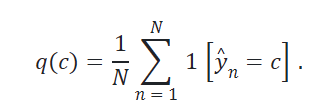
\includegraphics[width=0.62\linewidth,keepaspectratio]{figures/image1.png}
\end{center}

% --- DOCX block 009 ---
% Original: 其中，N 表示测试图像数量，c 表示诊断类别，q(c) 表示模型将测试图像预测为类别 c 的比例。进一步定义预测坍缩强度为：
Here, $N$ denotes the number of test images, $c$ denotes a diagnostic class, and $q(c)$ denotes the fraction of test images predicted as class $c$. We further define the prediction-collapse strength as:


% --- DOCX block 010 ---
% Original image: image2.png
\begin{center}
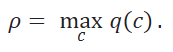
\includegraphics[width=0.62\linewidth,keepaspectratio]{figures/image2.png}
\end{center}

% --- DOCX block 011 ---
% Original: ρ 是预测分布中的最大类别占比；ρ 越接近 1，模型越接近单一类别预测器。
$\rho$ is the largest class proportion in the predicted distribution; the closer $\rho$ is to 1, the closer the model is to a single-class predictor.


% --- DOCX block 012 ---
% Original: 具体而言，在多中心医学图像任务中，每个客户端通常只观测到全局诊断空间的一个子集，因此本地模型不可避免地带有类别偏置。但这种偏置并不意味着客户端模型已经退化为单类预测器：融合前的本地模型仍可对多个诊断类别产生有效响应。退化主要出现在后置融合阶段。现有参数级融合方法以模型整体为单位进行平均、裁剪或符号聚合，缺乏对“客户端在哪些诊断类别上具有可靠判别能力”的显式刻画。因此，原本局部且可控的类别偏置在全局参数空间中被叠加和放大，最终形成融合模型的单类或少数类预测坍缩。
Specifically, in multi-center medical image tasks, each client usually observes only a subset of the global diagnostic space, so local models inevitably carry class bias. However, this bias does not mean that the client models have already degenerated into single-class predictors: before merging, local models can still respond effectively to multiple diagnostic classes. The degeneration mainly occurs during post-hoc merging. Existing parameter-level merging methods operate on whole models through averaging, pruning, or sign aggregation, and lack an explicit description of which diagnostic classes each client can discriminate reliably. As a result, originally local and controllable class bias is superposed and amplified in the global parameter space, eventually forming single-class or few-class predictive collapse in the merged model.


% --- DOCX block 013 ---
% Original: 以 OrgansMNIST-224、ResNet、3 clients、beta=0.01 为例，三个客户端的 ρ 分别为 0.7683、0.3161 和 0.3686，说明本地模型虽具有不同程度的类别偏置，但并未全部退化为单类输出。在相同设置下，Breadcrumbs 融合模型的 ρ 达到 0.9738，预测几乎集中到单一诊断类别。该结果说明，预测坍缩并非简单继承自已经失效的客户端模型，而是由类别无关的融合过程进一步诱发。
For example, on OrgansMNIST-224 with ResNet, 3 clients, and $\beta=0.01$, the three clients have $\rho$ values of 0.7683, 0.3161, and 0.3686, respectively. This indicates that local models have different degrees of class bias but have not all collapsed to a single output class. Under the same setting, the Breadcrumbs merged model reaches $\rho=0.9738$, with predictions almost concentrated on one diagnostic class. This result shows that predictive collapse is not simply inherited from already failed client models, but is further induced by a class-agnostic merging process.


% --- DOCX block 014 ---
% Original: 该观察直接引出 M1：后置融合不应只在参数空间中混合分类头，而应显式保存客户端仍然有效的类别级诊断知识。为此，M1 要求客户端上传每个诊断类别的特征原型，并以诊断原型作为本地判别能力的结构化载体。
This observation directly motivates M1: post-hoc merging should not only mix classifier heads in parameter space, but should explicitly preserve the class-level diagnostic knowledge that remains effective on clients. Therefore, M1 requires clients to upload feature prototypes for each diagnostic class, using diagnostic prototypes as structured carriers of local discriminative ability.


% --- DOCX block 015 ---
% Original: 观测 2：长尾先验下的坍缩收益（Collapse Benefit under Long-tailed Priors）。
\subsection{Observation 2: Collapse Benefit under Long-tailed Priors.}

% --- DOCX block 016 ---
% Original: 医学图像分类通常继承真实临床流行率或采样流行率，因而常见病、常见器官或高频诊断类别可能在测试集中占据较高比例。设测试集中最高频类别的占比为：
Medical image classification usually inherits real clinical prevalence or sampling prevalence, so common diseases, common organs, or high-frequency diagnostic classes may occupy a large proportion of the test set. Let the highest-frequency class proportion in the test set be:


% --- DOCX block 017 ---
% Original image: image3.png
\begin{center}
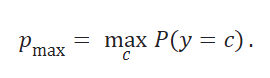
\includegraphics[width=0.62\linewidth,keepaspectratio]{figures/image3.png}
\end{center}

% --- DOCX block 018 ---
% Original: 如果一个模型完全坍缩到这个最高频类别，那么它虽然没有真正的多类别诊断能力，但仍可以得到如下 accuracy：
If a model completely collapses to this highest-frequency class, then it has no real multi-class diagnostic ability but can still obtain the following accuracy:


% --- DOCX block 019 ---
% Original image: image4.png
\begin{center}
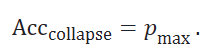
\includegraphics[width=0.62\linewidth,keepaspectratio]{figures/image4.png}
\end{center}

% --- DOCX block 020 ---
% Original: 因此，当最高频类别占比较大时，单类预测器可以在没有多类别诊断能力的情况下获得较高 accuracy。换言之，在长尾医学数据上，accuracy 可能将多数类坍缩误判为有效融合。这一现象解释了部分基线方法虽然预测分布高度集中，却仍能获得较高 accuracy 的原因。
Therefore, when the highest-frequency class proportion is large, a single-class predictor can obtain high accuracy without multi-class diagnostic ability. In other words, on long-tailed medical data, Accuracy may misinterpret majority-class collapse as effective merging. This phenomenon explains why some baselines can still obtain high Accuracy despite having highly concentrated prediction distributions.


% --- DOCX block 021 ---
% Original: 该观察引出 M2：消除坍缩并不等价于强制预测分布均匀化，因为医学数据中的长尾先验具有真实统计含义；同时，模型也不能退化为多数类预测器。M2 因此不改变 M1 已经重建出的诊断原型，而是在客户端上传的患病率计数显示存在强主导类别时，对分类分数加入有界的中心化 log-prior。这样既保留每个诊断类别的独立判别方向，又允许真实高频类别获得必要的 accuracy 校准。
This observation motivates M2: eliminating collapse is not equivalent to forcing the prediction distribution to become uniform, because long-tailed priors in medical data have real statistical meaning; at the same time, the model must not degenerate into a majority-class predictor. M2 therefore does not change the diagnostic prototypes reconstructed by M1. Instead, when prevalence counts uploaded by clients indicate a strong dominant class, M2 adds a bounded centered log-prior to the classification scores. This preserves the independent discriminative direction of each diagnostic class while allowing real high-frequency classes to receive necessary Accuracy calibration.


% --- DOCX block 022 ---
% Original: 相关工作
\section{Related Work}

% --- DOCX block 023 ---
% Original: Model Merging
\subsection{Model Merging}

% --- DOCX block 024 ---
% Original: 通用事后模型融合旨在整合已经训练完成的模型检查点，从而避免联合训练或重新训练带来的成本。现有方法可以按照融合变量进行归类。第一类方法直接在权重空间中插值，例如权重平均和 Model Soups；当多个模型仍处在兼容的参数盆地中时，这类方法能够取得较好的融合效果。第二类方法在参数增量空间中运算，例如 Task Arithmetic 将微调模型表示为相对于共享初始化模型的参数位移，并对这些位移进行线性组合。第三类方法试图在平均前消除参数干扰，例如 Git Re-Basin 通过神经元置换对齐减少排列不一致，TIES-Merging 和 DARE 系列方法通过裁剪微小更新、符号投票或随机丢弃并重缩放任务向量来缓解更新冲突。第四类方法进一步引入几何、曲率或鲁棒统计假设，例如 Fisher 融合、RegMean、Model Stock、Breadcrumbs、Iso-C、FreeMerge 和 RobustMerge。
General post-hoc model merging aims to integrate already trained checkpoints, thereby avoiding the cost of joint training or retraining. Existing methods can be categorized according to the variable being merged. The first class directly interpolates in weight space, such as weight averaging and Model Soups; these methods can perform well when multiple models remain within compatible parameter basins. The second class operates in parameter-delta space, for example Task Arithmetic represents fine-tuned models as parameter displacements relative to a shared initialization and linearly combines these displacements. The third class attempts to remove parameter interference before averaging; for example, Git Re-Basin reduces permutation mismatch through neuron permutation alignment, while TIES-Merging and the DARE family alleviate update conflicts through pruning small updates, sign voting, or randomly dropping and rescaling task vectors. The fourth class further introduces geometric, curvature, or robust statistical assumptions, such as Fisher merging, RegMean, Model Stock, Breadcrumbs, Iso-C, FreeMerge, and RobustMerge.


% --- DOCX block 025 ---
% Original: 这些方法构成本文的重要基线，但其融合变量并未针对医学诊断类别建模。它们操作的是全局参数、任务向量、曲率估计、置换结构或更新符号，而不是“客户端 (i) 是否在诊断类别 (c) 上拥有可靠证据”。在多中心医学图像任务中，客户端训练集通常同时存在类别缺失和长尾分布；当许多客户端-类别对满足 (n_{i,c}=0) 时，类别无关的参数融合会把某个客户端中可靠的类别方向与其他客户端中缺失或冲突的方向混合。结果是融合模型可能保留多数类方向，同时抑制罕见类或局部缺失类，形成预测分布高度集中的全局坍缩模型。
These methods form important baselines in this paper, but their merging variables do not model medical diagnostic classes. They operate on global parameters, task vectors, curvature estimates, permutation structures, or update signs, rather than on whether client $i$ has reliable evidence for diagnostic class $c$. In multi-center medical image tasks, client training sets usually contain both missing classes and long-tailed distributions. When many client-class pairs satisfy $n_{i,c}=0$, class-agnostic parameter merging mixes a reliable class direction from one client with missing or conflicting directions from other clients. Consequently, the merged model may retain majority-class directions while suppressing rare or locally missing classes, leading to a globally collapsed model with a highly concentrated prediction distribution.


% --- DOCX block 026 ---
% Original: 因此，通用融合方法在本文场景下失效的关键并非其参数融合技术本身不充分，而是其融合变量与多中心医学数据的核心结构不匹配。医学图像融合需要显式表示类别级诊断可及性，即每个客户端对不同诊断类别的证据强度不同。LAMP-Merge 的 M1 正是针对这一缺口设计：它不直接平均分类头，而是由客户端上传类别原型和类别支持数，并在服务端按类别重建全局诊断原型分类器。
Therefore, the key reason why general merging methods fail in our setting is not that their parameter-merging techniques are intrinsically weak, but that their merging variables are mismatched with the core structure of multi-center medical data. Medical image merging needs to explicitly represent class-level diagnostic availability, namely that each client has different evidence strength for different diagnostic classes. M1 in LAMP-Merge is designed precisely for this gap: it does not directly average classifier heads, but lets clients upload class prototypes and class support counts, and reconstructs a global diagnostic prototype classifier class by class on the server.


% --- DOCX block 027 ---
% Original: Medical Model Merging
\subsection{Medical Model Merging}

% --- DOCX block 028 ---
% Original: 医学融合方法通常利用临床数据中特有的结构。例如，mTAN 使用连续时间注意力处理非规则采样时间序列，Raindrop 使用图结构建模生理传感器之间的关系，MedFuse 将胸片图像与临床时间序列进行融合。这些工作表明，医学数据不是通用融合算法的简单应用场景；医学数据具有非规则时间结构、模态异质性、临床测量机制以及疾病患病率分布等特征。
Medical fusion methods usually exploit structures specific to clinical data. For example, mTAN uses continuous-time attention for irregularly sampled time series, Raindrop uses graph structures to model relationships among physiological sensors, and MedFuse fuses chest X-ray images with clinical time series. These works show that medical data are not merely application scenarios for general fusion algorithms; medical data have irregular temporal structure, modality heterogeneity, clinical measurement mechanisms, and disease-prevalence distributions.


% --- DOCX block 029 ---
% Original: 然而，这类医学融合方法通常融合的是患者级输入模态或临床表征，而不是独立训练后的医学图像分类器检查点。其训练过程往往需要访问患者级样本、时间戳、多模态记录、EHR 或服务器端验证反馈。当服务器不能查看客户端原始医学图像、逐样本特征、逐样本 logit 或逐样本预测时，这类方法不能直接用于本文的一次性模型融合设定。
However, these medical fusion methods usually fuse patient-level input modalities or clinical representations, rather than independently trained medical image classifier checkpoints. Their training processes often require access to patient-level samples, timestamps, multimodal records, EHR, or server-side validation feedback. When the server cannot view clients' raw medical images, per-sample features, per-sample logits, or per-sample predictions, these methods cannot be directly applied to the one-shot model-merging setting studied in this paper.


% --- DOCX block 030 ---
% Original: 而不泄露原图的模型融合算法，如MedMerge(https://ieeexplore.ieee.org/abstract/document/11382027/)，则...
Model-merging algorithms that do not leak raw images, such as MedMerge (https://ieeexplore.ieee.org/abstract/document/11382027/), then ...


% --- DOCX block 031 ---
% Original: LAMP-Merge 将医学结构限定在可上传的类别级统计中：客户端本地计算诊断类别原型和患病率计数，服务端只基于这些聚合统计完成模型构造。因此，它不需要访问用户的图像来源，保护了患者的隐私。
LAMP-Merge confines medical structure to uploadable class-level statistics: clients locally compute diagnostic class prototypes and prevalence counts, and the server constructs the model only from these aggregate statistics. Therefore, it does not need access to the source images, preserving patient privacy.


% --- DOCX block 032 ---
% Original: Federated Learning
\subsection{Federated Learning}

% --- DOCX block 033 ---
% Original: 联邦学习和去中心化学习是隐私敏感医学人工智能中的重要研究方向。FedAvg 及其变体通过多轮通信训练全局模型：服务器下发模型，客户端执行本地优化，随后上传更新并由服务器聚合。Swarm Learning 去除了传统中心参数服务器，利用去中心化协调机制实现多方训练。Gossip Learning 进一步以点对点方式异步传播模型，使参与者在局部训练和模型交换中逐步获得协作收益。这些方法适用于客户端能够长期在线、反复通信并根据中间全局模型继续训练的场景。然而，本文研究的问题并不是协作训练，而是训练完成后的单次异步合并。现实医疗部署中，不同医院可能在不同时间完成训练，且难以承担反复下发、训练和回传的协议成本。因此，本文设定中服务器不会向客户端发送一系列全局模型，客户端也不会在观察服务器聚合结果后继续优化。由此可见，联邦学习和去中心化学习解决的是多轮训练协议问题，而 LAMP-Merge 解决的是一次性事后融合问题。LAMP-Merge 只要求客户端在本地训练结束后上传一次模型和类别级统计；服务端在不建立多轮反馈闭环的情况下生成一个统一全局诊断模型。
Federated learning and decentralized learning are important directions in privacy-sensitive medical AI. FedAvg and its variants train a global model through multiple communication rounds: the server sends a model, clients perform local optimization, then upload updates for server aggregation. Swarm Learning removes the traditional central parameter server and uses decentralized coordination for multi-party training. Gossip Learning further propagates models asynchronously in a peer-to-peer manner, allowing participants to gradually obtain collaborative benefits through local training and model exchange. These methods are suitable when clients can remain online for a long time, communicate repeatedly, and continue training from intermediate global models. However, the problem studied in this paper is not collaborative training, but single-shot asynchronous merging after training is complete. In realistic medical deployment, hospitals may finish training at different times and may not be able to afford repeated model distribution, training, and upload protocols. Therefore, in our setting, the server does not send a sequence of global models to clients, and clients do not continue optimization after observing the server's merged result. Thus, federated learning and decentralized learning solve multi-round training-protocol problems, while LAMP-Merge solves the one-shot post-hoc merging problem. LAMP-Merge only requires each client to upload its model and class-level statistics once after local training, and the server generates a unified global diagnostic model without establishing a multi-round feedback loop.


% --- DOCX block 034 ---
% Original: 方法设计
\section{Method Design}

% --- DOCX block 035 ---
% Original: 模块1：原型重建模块
\subsection{Module 1: Prototype Reconstruction Module}

% --- DOCX block 036 ---
% Original: 针对医学模型融合中，后置参数融合会退化为预测分布高度集中的全局坍缩模型的问题，我们提出了原型重建模块，旨在通过依据分布重定义权重来缓解坍缩问题。
To address the problem that post-hoc parameter merging can degenerate into a globally collapsed model with a highly concentrated prediction distribution in medical model merging, we propose the prototype reconstruction module, which aims to mitigate collapse by redefining weights according to the data distribution.


% --- DOCX block 037 ---
% Original: LAMP-Merge首先在共享的参考特征空间中重建按类别划分的诊断头部模型。设为本地训练前从共享模型配置中实例化的固定参考骨干网络，T（·）为评估变 
LAMP-Merge first reconstructs a class-wise diagnostic head in the shared reference feature space. Let the fixed reference backbone be instantiated from the shared model configuration before local training, and let $T(\cdot)$ be the evaluation transform.

% Original image: image5.png
\begin{center}
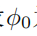
\includegraphics[width=0.62\linewidth,keepaspectratio]{figures/image5.png}
\end{center}

% --- DOCX block 038 ---
% Original: 换函数。对于每个诊断类别c，客户端i均计算出对应的 
For each diagnostic class $c$, client $i$ computes the corresponding


% --- DOCX block 039 ---
% Original: 参考空间类别原型。 
reference-space class prototype.


% --- DOCX block 040 ---
% Original image: image6.png
\begin{center}
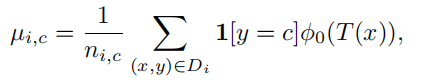
\includegraphics[width=0.62\linewidth,keepaspectratio]{figures/image6.png}
\end{center}

% --- DOCX block 041 ---
% Original: 其中表示该类别的支持数量。若ni,c= 0，则客户端对该类别未上传任何支持数据，亦未提供原型证据。 
Here, the term denotes the support size of this class. If $n_{i,c}=0$, then the client uploads no support data for this class and provides no prototype evidence.

% Original image: image7.png
\begin{center}
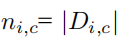
\includegraphics[width=0.62\linewidth,keepaspectratio]{figures/image7.png}
\end{center}

% --- DOCX block 042 ---
% Original: 服务器将支持计数转换为证据权重： 
The server converts support counts into evidence weights:


% --- DOCX block 043 ---
% Original: 为 
where

% Original image: image8.png
\begin{center}
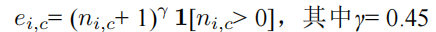
\includegraphics[width=0.62\linewidth,keepaspectratio]{figures/image8.png}
\end{center}

% --- DOCX block 044 ---
% Original: 默认证据指数。客户端i对类别c的归一化可靠性为 
is the default evidence exponent. The normalized reliability of client $i$ for class $c$ is


% --- DOCX block 045 ---
% Original image: image9.png
\begin{center}
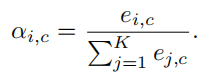
\includegraphics[width=0.62\linewidth,keepaspectratio]{figures/image9.png}
\end{center}

% --- DOCX block 046 ---
% Original: 随后，诊断原型被建立为。 
Then the diagnostic prototype is constructed as


% --- DOCX block 047 ---
% Original image: image10.png
\begin{center}
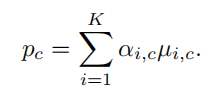
\includegraphics[width=0.62\linewidth,keepaspectratio]{figures/image10.png}
\end{center}

% --- DOCX block 048 ---
% Original: 最后，LAMP-Merge算法可合成一个余弦原型分类器： 
Finally, LAMP-Merge synthesizes a cosine prototype classifier:


% --- DOCX block 049 ---
% Original image: image11.png
\begin{center}
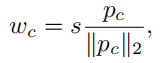
\includegraphics[width=0.62\linewidth,keepaspectratio]{figures/image11.png}
\end{center}

% --- DOCX block 050 ---
% Original: 其中s=20为默认头部规模。
where $s=20$ is the default head scale.


% --- DOCX block 051 ---
% Original: 该模块并非对不兼容的分类器头部进行平均处理，而是保留每个客户端均具备证据支持的类别，并重建全局多类诊断头部。
This module does not average incompatible classifier heads. Instead, it preserves the classes for which each client has evidence support and reconstructs a global multi-class diagnostic head.


% --- DOCX block 052 ---
% Original: 模块2：长尾率校准模块
\subsection{Module 2: Long-tail Prevalence Calibration Module}

% --- DOCX block 053 ---
% Original: 模块2应该对应问题2.
Module 2 should correspond to Question 2.


% --- DOCX block 054 ---
% Original: 参考：针对医学模型融合中，长尾分布存在坍缩收益的问题，我们提出了长尾率校准模块，旨在通过增加类型先验知识来缓解该问题。
Reference: To address the collapse benefit caused by long-tailed distributions in medical model merging, we propose the long-tail prevalence calibration module, which aims to mitigate this issue by adding class-prior knowledge.


% --- DOCX block 055 ---
% Original: 每个客户端还需上传各类别的患病率 
Each client also uploads the prevalence


% --- DOCX block 056 ---
% Original: 计数值 。服务器则据此估算全局类别的先验分布。
count value for each class. The server then estimates the global class prior distribution.


% --- DOCX block 057 ---
% Original image: image12.png
\begin{center}
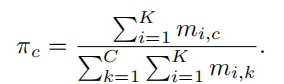
\includegraphics[width=0.62\linewidth,keepaspectratio]{figures/image12.png}
\end{center}

% --- DOCX block 058 ---
% Original: 我们通过以下方式衡量主导阶层的失衡状况： 
We measure the imbalance of the dominant class as follows:


% --- DOCX block 059 ---
% Original: ,C是类别总数
where $C$ is the total number of classes.

% Original image: image13.png
\begin{center}
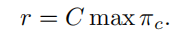
\includegraphics[width=0.62\linewidth,keepaspectratio]{figures/image13.png}
\end{center}

% --- DOCX block 060 ---
% Original: M2仅在r > τ时被激活（默认情况下τ= 2.5）。激活后，它会添加一个居中的对数先验偏置项。 
M2 is activated only when $r>\tau$ (default $\tau=2.5$). Once activated, it adds a centered log-prior bias term.


% --- DOCX block 061 ---
% Original image: image14.png
\begin{center}
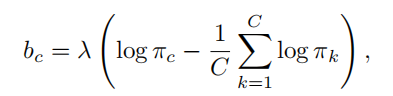
\includegraphics[width=0.62\linewidth,keepaspectratio]{figures/image14.png}
\end{center}

% --- DOCX block 062 ---
% Original: 默认最大校准强度λ=5.0。最终得分为 
The default maximum calibration strength is $\lambda=5.0$. The final score is


% --- DOCX block 063 ---
% Original image: image15.png
\begin{center}
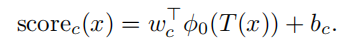
\includegraphics[width=0.62\linewidth,keepaspectratio]{figures/image15.png}
\end{center}

% --- DOCX block 064 ---
% Original: 实验设计
\section{Experimental Design}

% --- DOCX block 065 ---
% Original:   我们在单次异步医学模型融合场景下评估LAMP-Merge算法。每个客户端在其私有且具有类别偏好的数据分区上进行本地训练；完成本地训练后，客户端上传一个检查点及LAMP-Merge所需的类别级统计信息。服务器仅执行一次数据合并操作，并不运行迭代式的服务器-客户端优化流程。
We evaluate LAMP-Merge in a single-shot asynchronous medical model-merging scenario. Each client trains locally on its private and class-biased data partition. After local training is complete, each client uploads one checkpoint and the class-level statistics required by LAMP-Merge. The server performs only one merging operation and does not run an iterative server-client optimization process.


% --- DOCX block 066 ---
% Original: /*
\begin{quote}\small /*\end{quote}

% --- DOCX block 067 ---
% Original: 医学图像
\begin{quote}\small Medical images\end{quote}

% --- DOCX block 068 ---
% Original:   + 多客户端已训练 checkpoint
\begin{quote}\small + multiple trained client checkpoints\end{quote}

% --- DOCX block 069 ---
% Original:   + 服务端不看 raw data / validation data / proxy data
\begin{quote}\small + the server does not view raw data / validation data / proxy data\end{quote}

% --- DOCX block 070 ---
% Original:   + 不把候选模型发回客户端打分
\begin{quote}\small + candidate models are not sent back to clients for scoring\end{quote}

% --- DOCX block 071 ---
% Original:   + single-shot post-hoc model merging
\begin{quote}\small + single-shot post-hoc model merging\end{quote}

% --- DOCX block 072 ---
% Original: 客户端本地计算统计，服务端只融合统计和 checkpoint。设计重点尝试放在客户端上，用最少隐私的泄露给出最好的性能。
\begin{quote}\small Clients compute statistics locally, and the server only merges statistics and checkpoints. The design emphasis is placed on the client side, using minimal privacy exposure to obtain the best possible performance.\end{quote}

% --- DOCX block 073 ---
% Original:     原因：在客户端的有限数据中，难以找到一个方法用来结合这些客户端给出的信息。无论是增量融合、BN估计还是其他的一些方法，都会因为隐私保护->数据不足->评估不全面而导致最终性能甚至不如avg。
\begin{quote}\small Reason: within the limited data of each client, it is difficult to find a method that effectively combines the information provided by these clients. Whether using incremental fusion, BN estimation, or other methods, privacy protection leads to insufficient data, insufficient evaluation coverage, and final performance that can even be worse than avg.\end{quote}

% --- DOCX block 074 ---
% Original: */
\begin{quote}\small */\end{quote}

% --- DOCX block 075 ---
% Original: 实验设计矩阵：
\subsection{Experimental Design Matrix:}

% --- DOCX block 076 ---
% Original: 本文实验聚焦 医学模型融合 场景。
This paper focuses on the medical model-merging scenario.


% --- DOCX block 077 ---
% Original: 基础训练设置
\subsubsection{Basic Training Settings}

% --- DOCX block 078 ---
% Original: 数据集：我们使用了五个分辨率为224的医学图像分类数 
Datasets: We use five medical image classification datasets


% --- DOCX block 079 ---
% Original: 据集。所有任务均为单标签多类诊断或器官识别任务。
with resolution 224. All tasks are single-label multi-class diagnosis or organ-recognition tasks.


% --- DOCX block 080 ---
% Original: 对于标准视觉模型架构，我们评估了ResNet、ConvNeXt、ViT-Tiny和Swin-Tiny；对于视觉-语言模型，则评估了openai/clip-vit-base-patch32。针对每组数据集-模 型组合，我们构建了非 IID 客户端划分方案，其中客户端 数 量 K∈{3,5,7}，β ∈{0,0.01,0.1}。所有实验结果均使用种子值42。该基准测试包含225个原始测试准确率单元和75个客户端平均单元；客户端平均指标通过计算固定客户端数量下三个β值的平均值，从而降低对单一划分偏斜度的敏感性。
For standard vision model architectures, we evaluate ResNet, ConvNeXt, ViT-Tiny, and Swin-Tiny; for the vision-language model, we evaluate openai/clip-vit-base-patch32. For each dataset-model combination, we construct non-IID client partitions with the number of clients $K\in\{3,5,7\}$ and $\beta\in\{0,0.01,0.1\}$. All experiments use seed 42. This benchmark contains 225 raw test-accuracy cells and 75 client-average cells; the client-average metric averages the three $\beta$ values under a fixed client number, reducing sensitivity to a single partition skewness.


% --- DOCX block 081 ---
% Original: Backbone 设置
\subsubsection{Backbone Settings}

% --- DOCX block 082 ---
% Original: “共享参考特征空间”是由共享参考骨干网络 phi_0 和预处理 T 产生的特征坐标系。
The shared reference feature space is the feature coordinate system produced by the shared reference backbone $\phi_0$ and preprocessing transform $T$.


% --- DOCX block 083 ---
% Original: 我们与十二种事后合并基线方法进行了比较： avg、ties、dare__linear、dare__ties、regmean、fisher、breadcrumb、model__stock、from、 iso__c 、free__merge 和 robustmerge。主要比较标准为：当LAMPMerge值大于或等于该单元格中最强的非LAMP基线方法时，即判定该单元格的合并结果成功。
We compare against twelve post-hoc merging baselines: avg, ties, dare\_linear, dare\_ties, regmean, fisher, breadcrumb, model\_stock, from, iso\_c, free\_merge, and robustmerge. The main comparison criterion is that a cell is counted as successful if the LAMP-Merge value is greater than or equal to the strongest non-LAMP baseline in that cell.


% --- DOCX block 084 ---
% Original: All experiments were run on a server with two Intel(R) Xeon(R) Silver 4210 CPUs @ 2.20GHz, 40 logical CPU threads in total, and four NVIDIA GeForce RTX 2080 Ti GPUs with 11264 MiB memory each. The NVIDIA driver version is 535.154.05. The operating system is Ubuntu 20.04.1 LTS. The software environment is the conda environment \texttt{MM}, using Python 3.10.20, PyTorch 2.6.0+\texttt{cu118}, torchvision 0.21.0+\texttt{cu118}, NumPy 2.2.6, and CUDA runtime 11.8.
All experiments were run on a server with two Intel(R) Xeon(R) Silver 4210 CPUs @ 2.20GHz, 40 logical CPU threads in total, and four NVIDIA GeForce RTX 2080 Ti GPUs with 11264 MiB memory each. The NVIDIA driver version is 535.154.05. The operating system is Ubuntu 20.04.1 LTS. The software environment is the conda environment \texttt{MM}, using Python 3.10.20, PyTorch 2.6.0+\texttt{cu118}, torchvision 0.21.0+\texttt{cu118}, NumPy 2.2.6, and CUDA runtime 11.8.


% --- DOCX block 085 ---
% Original: 实验结果表格
\section{Experimental Result Tables}

% --- DOCX block 086 ---
% Original: Small
\subsection{Small}

% --- DOCX block 087 ---
% Original: resnet
\subsubsection{ResNet}

% --- DOCX block 088 ---
% Original: Client Average
Client Average


% --- DOCX block 089 ---
% Original table row: method | bloodmnist_224 | dermamnist_224 | organcmnist_224 | organsmnist_224 | chaoshengmnist_224
% Original table row:  | c3_avg | c5_avg | c7_avg | c3_avg | c5_avg | c7_avg | c3_avg | c5_avg | c7_avg | c3_avg | c5_avg | c7_avg | c3_avg | c5_avg | c7_avg
% Original table row: avg | 0.3345 | 0.2467 | 0.2822 | 0.6291 | 0.4700 | 0.6244 | 0.2261 | 0.1772 | 0.1396 | 0.2864 | 0.1794 | 0.2475 | 0.2435 | 0.1581 | 0.1542
% Original table row: ties | 0.2601 | 0.1872 | 0.1787 | 0.5995 | 0.4841 | 0.6484 | 0.2650 | 0.1684 | 0.2118 | 0.1981 | 0.1915 | 0.1874 | 0.3477 | 0.1989 | 0.1854
% Original table row: dare_linear | 0.2832 | 0.2856 | 0.2392 | 0.6357 | 0.4841 | 0.6288 | 0.2018 | 0.2588 | 0.1650 | 0.2545 | 0.2245 | 0.2537 | 0.2162 | 0.1728 | 0.1608
% Original table row: dare_ties | 0.3194 | 0.1935 | 0.1780 | 0.5375 | 0.4825 | 0.5558 | 0.1851 | 0.1515 | 0.1859 | 0.1790 | 0.1352 | 0.1730 | 0.2932 | 0.1635 | 0.1890
% Original table row: regmean | 0.3460 | 0.2369 | 0.3407 | 0.5812 | 0.2843 | 0.5022 | 0.2405 | 0.1340 | 0.1388 | 0.2504 | 0.1623 | 0.1493 | 0.2276 | 0.1695 | 0.1318
% Original table row: fisher | 0.3196 | 0.2237 | 0.2608 | 0.6707 | 0.6702 | 0.6690 | 0.2973 | 0.1741 | 0.1812 | 0.2010 | 0.2956 | 0.1963 | 0.2333 | 0.1860 | 0.2513
% Original table row: breadcrumbs | 0.0854 | 0.1417 | 0.1460 | 0.0495 | 0.2913 | 0.1721 | 0.0766 | 0.0676 | 0.0685 | 0.0802 | 0.0948 | 0.0603 | 0.1225 | 0.1273 | 0.1021
% Original table row: model_stock | 0.2420 | 0.1824 | 0.1975 | 0.6216 | 0.4311 | 0.5721 | 0.1225 | 0.1274 | 0.1185 | 0.2742 | 0.1578 | 0.2012 | 0.1791 | 0.1321 | 0.1578
% Original table row: from | 0.2989 | 0.2306 | 0.2052 | 0.6713 | 0.4369 | 0.6580 | 0.2350 | 0.1560 | 0.1520 | 0.2207 | 0.2087 | 0.2476 | 0.2309 | 0.1506 | 0.2063
% Original table row: iso_c | 0.3278 | 0.2748 | 0.3023 | 0.5049 | 0.4422 | 0.6416 | 0.2331 | 0.1629 | 0.1383 | 0.2736 | 0.2118 | 0.2453 | 0.2615 | 0.1698 | 0.1554
% Original table row: free_merge | 0.3345 | 0.2467 | 0.2822 | 0.6291 | 0.4700 | 0.6246 | 0.2261 | 0.1771 | 0.1396 | 0.2863 | 0.1793 | 0.2475 | 0.2435 | 0.1581 | 0.1545
% Original table row: robustmerge | 0.3401 | 0.2430 | 0.2256 | 0.2956 | 0.2085 | 0.3942 | 0.2458 | 0.1764 | 0.1653 | 0.2680 | 0.2227 | 0.2301 | 0.2189 | 0.2231 | 0.1707
% Original table row: LAMP-Merge | 0.8000 | 0.7987 | 0.7984 | 0.6732 | 0.6736 | 0.6733 | 0.5930 | 0.5908 | 0.5905 | 0.5197 | 0.5191 | 0.5132 | 0.4804 | 0.4642 | 0.4714
\begin{table*}[t]
\centering
\scriptsize
\setlength{\tabcolsep}{2pt}
\resizebox{\textwidth}{!}{%
\begin{tabular}{lccccccccccccccc}
\toprule
Method & bloodmnist\_224 & dermamnist\_224 & organcmnist\_224 & organsmnist\_224 & chaoshengmnist\_224 &  &  &  &  &  &  &  &  &  &  \\
\midrule
 & c3\_avg & c5\_avg & c7\_avg & c3\_avg & c5\_avg & c7\_avg & c3\_avg & c5\_avg & c7\_avg & c3\_avg & c5\_avg & c7\_avg & c3\_avg & c5\_avg & c7\_avg \\
\midrule
avg & 0.3345 & 0.2467 & 0.2822 & 0.6291 & 0.4700 & 0.6244 & 0.2261 & 0.1772 & 0.1396 & 0.2864 & 0.1794 & 0.2475 & 0.2435 & 0.1581 & 0.1542 \\
ties & 0.2601 & 0.1872 & 0.1787 & 0.5995 & 0.4841 & 0.6484 & 0.2650 & 0.1684 & 0.2118 & 0.1981 & 0.1915 & 0.1874 & 0.3477 & 0.1989 & 0.1854 \\
dare\_linear & 0.2832 & 0.2856 & 0.2392 & 0.6357 & 0.4841 & 0.6288 & 0.2018 & 0.2588 & 0.1650 & 0.2545 & 0.2245 & 0.2537 & 0.2162 & 0.1728 & 0.1608 \\
dare\_ties & 0.3194 & 0.1935 & 0.1780 & 0.5375 & 0.4825 & 0.5558 & 0.1851 & 0.1515 & 0.1859 & 0.1790 & 0.1352 & 0.1730 & 0.2932 & 0.1635 & 0.1890 \\
regmean & 0.3460 & 0.2369 & 0.3407 & 0.5812 & 0.2843 & 0.5022 & 0.2405 & 0.1340 & 0.1388 & 0.2504 & 0.1623 & 0.1493 & 0.2276 & 0.1695 & 0.1318 \\
fisher & 0.3196 & 0.2237 & 0.2608 & 0.6707 & 0.6702 & 0.6690 & 0.2973 & 0.1741 & 0.1812 & 0.2010 & 0.2956 & 0.1963 & 0.2333 & 0.1860 & 0.2513 \\
breadcrumbs & 0.0854 & 0.1417 & 0.1460 & 0.0495 & 0.2913 & 0.1721 & 0.0766 & 0.0676 & 0.0685 & 0.0802 & 0.0948 & 0.0603 & 0.1225 & 0.1273 & 0.1021 \\
model\_stock & 0.2420 & 0.1824 & 0.1975 & 0.6216 & 0.4311 & 0.5721 & 0.1225 & 0.1274 & 0.1185 & 0.2742 & 0.1578 & 0.2012 & 0.1791 & 0.1321 & 0.1578 \\
from & 0.2989 & 0.2306 & 0.2052 & 0.6713 & 0.4369 & 0.6580 & 0.2350 & 0.1560 & 0.1520 & 0.2207 & 0.2087 & 0.2476 & 0.2309 & 0.1506 & 0.2063 \\
iso\_c & 0.3278 & 0.2748 & 0.3023 & 0.5049 & 0.4422 & 0.6416 & 0.2331 & 0.1629 & 0.1383 & 0.2736 & 0.2118 & 0.2453 & 0.2615 & 0.1698 & 0.1554 \\
free\_merge & 0.3345 & 0.2467 & 0.2822 & 0.6291 & 0.4700 & 0.6246 & 0.2261 & 0.1771 & 0.1396 & 0.2863 & 0.1793 & 0.2475 & 0.2435 & 0.1581 & 0.1545 \\
robustmerge & 0.3401 & 0.2430 & 0.2256 & 0.2956 & 0.2085 & 0.3942 & 0.2458 & 0.1764 & 0.1653 & 0.2680 & 0.2227 & 0.2301 & 0.2189 & 0.2231 & 0.1707 \\
LAMP-Merge & 0.8000 & 0.7987 & 0.7984 & 0.6732 & 0.6736 & 0.6733 & 0.5930 & 0.5908 & 0.5905 & 0.5197 & 0.5191 & 0.5132 & 0.4804 & 0.4642 & 0.4714 \\
\bottomrule
\end{tabular}%
}
\end{table*}

% --- DOCX block 090 ---
% Original: convnext
\subsubsection{ConvNeXt}

% --- DOCX block 091 ---
% Original table row: method | bloodmnist_224 | dermamnist_224 | organcmnist_224 | organsmnist_224 | chaoshengmnist_224
% Original table row:  | c3_avg | c5_avg | c7_avg | c3_avg | c5_avg | c7_avg | c3_avg | c5_avg | c7_avg | c3_avg | c5_avg | c7_avg | c3_avg | c5_avg | c7_avg
% Original table row: avg | 0.1565 | 0.1122 | 0.1384 | 0.2966 | 0.4830 | 0.6688 | 0.1037 | 0.1218 | 0.0944 | 0.1308 | 0.1035 | 0.1416 | 0.1506 | 0.1506 | 0.1252
% Original table row: ties | 0.1715 | 0.1214 | 0.1524 | 0.2966 | 0.1797 | 0.2713 | 0.1217 | 0.0786 | 0.0716 | 0.1123 | 0.0761 | 0.0796 | 0.1518 | 0.1456 | 0.1291
% Original table row: dare_linear | 0.1756 | 0.1122 | 0.1345 | 0.2705 | 0.4830 | 0.4830 | 0.1035 | 0.0699 | 0.1085 | 0.1282 | 0.1035 | 0.0797 | 0.1575 | 0.1575 | 0.1264
% Original table row: dare_ties | 0.1096 | 0.1519 | 0.1497 | 0.0908 | 0.2798 | 0.2451 | 0.1305 | 0.1346 | 0.0770 | 0.1096 | 0.0946 | 0.0709 | 0.1456 | 0.1297 | 0.1500
% Original table row: regmean | 0.1565 | 0.0817 | 0.1856 | 0.2633 | 0.0773 | 0.2720 | 0.1143 | 0.1017 | 0.0768 | 0.1014 | 0.1259 | 0.1038 | 0.1575 | 0.1539 | 0.1500
% Original table row: fisher | 0.1565 | 0.0999 | 0.1189 | 0.4825 | 0.2638 | 0.2971 | 0.1003 | 0.0974 | 0.0915 | 0.0604 | 0.0517 | 0.0843 | 0.1695 | 0.1360 | 0.1456
% Original table row: breadcrumbs | 0.1516 | 0.1366 | 0.1163 | 0.0524 | 0.2766 | 0.4630 | 0.1031 | 0.1444 | 0.1574 | 0.1516 | 0.1554 | 0.2077 | 0.1384 | 0.1363 | 0.1363
% Original table row: model_stock | 0.1756 | 0.1144 | 0.1778 | 0.2966 | 0.4830 | 0.6688 | 0.1276 | 0.1218 | 0.1385 | 0.1308 | 0.1035 | 0.1935 | 0.1575 | 0.1291 | 0.1479
% Original table row: from | 0.1565 | 0.1083 | 0.1671 | 0.2966 | 0.3406 | 0.4569 | 0.1232 | 0.1224 | 0.0650 | 0.1324 | 0.1105 | 0.0897 | 0.1575 | 0.1578 | 0.1087
% Original table row: iso_c | 0.1947 | 0.1865 | 0.1480 | 0.2971 | 0.4830 | 0.6688 | 0.0991 | 0.0699 | 0.0945 | 0.0789 | 0.1477 | 0.0867 | 0.1518 | 0.1291 | 0.1605
% Original table row: free_merge | 0.1575 | 0.1190 | 0.1384 | 0.2971 | 0.4830 | 0.6688 | 0.0906 | 0.1218 | 0.1385 | 0.1308 | 0.1035 | 0.1416 | 0.1506 | 0.1291 | 0.1695
% Original table row: robustmerge | 0.1410 | 0.1405 | 0.0752 | 0.0908 | 0.4507 | 0.4830 | 0.1394 | 0.1218 | 0.1793 | 0.2354 | 0.0961 | 0.2077 | 0.1300 | 0.1135 | 0.1363
% Original table row: LAMP-Merge | 0.8480 | 0.8476 | 0.8488 | 0.6033 | 0.5930 | 0.5987 | 0.6525 | 0.6501 | 0.6517 | 0.6062 | 0.6060 | 0.6071 | 0.4280 | 0.4283 | 0.4172
\begin{table*}[t]
\centering
\scriptsize
\setlength{\tabcolsep}{2pt}
\resizebox{\textwidth}{!}{%
\begin{tabular}{lccccccccccccccc}
\toprule
Method & bloodmnist\_224 & dermamnist\_224 & organcmnist\_224 & organsmnist\_224 & chaoshengmnist\_224 &  &  &  &  &  &  &  &  &  &  \\
\midrule
 & c3\_avg & c5\_avg & c7\_avg & c3\_avg & c5\_avg & c7\_avg & c3\_avg & c5\_avg & c7\_avg & c3\_avg & c5\_avg & c7\_avg & c3\_avg & c5\_avg & c7\_avg \\
\midrule
avg & 0.1565 & 0.1122 & 0.1384 & 0.2966 & 0.4830 & 0.6688 & 0.1037 & 0.1218 & 0.0944 & 0.1308 & 0.1035 & 0.1416 & 0.1506 & 0.1506 & 0.1252 \\
ties & 0.1715 & 0.1214 & 0.1524 & 0.2966 & 0.1797 & 0.2713 & 0.1217 & 0.0786 & 0.0716 & 0.1123 & 0.0761 & 0.0796 & 0.1518 & 0.1456 & 0.1291 \\
dare\_linear & 0.1756 & 0.1122 & 0.1345 & 0.2705 & 0.4830 & 0.4830 & 0.1035 & 0.0699 & 0.1085 & 0.1282 & 0.1035 & 0.0797 & 0.1575 & 0.1575 & 0.1264 \\
dare\_ties & 0.1096 & 0.1519 & 0.1497 & 0.0908 & 0.2798 & 0.2451 & 0.1305 & 0.1346 & 0.0770 & 0.1096 & 0.0946 & 0.0709 & 0.1456 & 0.1297 & 0.1500 \\
regmean & 0.1565 & 0.0817 & 0.1856 & 0.2633 & 0.0773 & 0.2720 & 0.1143 & 0.1017 & 0.0768 & 0.1014 & 0.1259 & 0.1038 & 0.1575 & 0.1539 & 0.1500 \\
fisher & 0.1565 & 0.0999 & 0.1189 & 0.4825 & 0.2638 & 0.2971 & 0.1003 & 0.0974 & 0.0915 & 0.0604 & 0.0517 & 0.0843 & 0.1695 & 0.1360 & 0.1456 \\
breadcrumbs & 0.1516 & 0.1366 & 0.1163 & 0.0524 & 0.2766 & 0.4630 & 0.1031 & 0.1444 & 0.1574 & 0.1516 & 0.1554 & 0.2077 & 0.1384 & 0.1363 & 0.1363 \\
model\_stock & 0.1756 & 0.1144 & 0.1778 & 0.2966 & 0.4830 & 0.6688 & 0.1276 & 0.1218 & 0.1385 & 0.1308 & 0.1035 & 0.1935 & 0.1575 & 0.1291 & 0.1479 \\
from & 0.1565 & 0.1083 & 0.1671 & 0.2966 & 0.3406 & 0.4569 & 0.1232 & 0.1224 & 0.0650 & 0.1324 & 0.1105 & 0.0897 & 0.1575 & 0.1578 & 0.1087 \\
iso\_c & 0.1947 & 0.1865 & 0.1480 & 0.2971 & 0.4830 & 0.6688 & 0.0991 & 0.0699 & 0.0945 & 0.0789 & 0.1477 & 0.0867 & 0.1518 & 0.1291 & 0.1605 \\
free\_merge & 0.1575 & 0.1190 & 0.1384 & 0.2971 & 0.4830 & 0.6688 & 0.0906 & 0.1218 & 0.1385 & 0.1308 & 0.1035 & 0.1416 & 0.1506 & 0.1291 & 0.1695 \\
robustmerge & 0.1410 & 0.1405 & 0.0752 & 0.0908 & 0.4507 & 0.4830 & 0.1394 & 0.1218 & 0.1793 & 0.2354 & 0.0961 & 0.2077 & 0.1300 & 0.1135 & 0.1363 \\
LAMP-Merge & 0.8480 & 0.8476 & 0.8488 & 0.6033 & 0.5930 & 0.5987 & 0.6525 & 0.6501 & 0.6517 & 0.6062 & 0.6060 & 0.6071 & 0.4280 & 0.4283 & 0.4172 \\
\bottomrule
\end{tabular}%
}
\end{table*}

% --- DOCX block 092 ---
% Original: Vit_t
\subsubsection{ViT-Tiny}

% --- DOCX block 093 ---
% Original: Client Average
Client Average


% --- DOCX block 094 ---
% Original table row: method | bloodmnist_224 | dermamnist_224 | organcmnist_224 | organsmnist_224 | chaoshengmnist_224
% Original table row:  | c3_avg | c5_avg | c7_avg | c3_avg | c5_avg | c7_avg | c3_avg | c5_avg | c7_avg | c3_avg | c5_avg | c7_avg | c3_avg | c5_avg | c7_avg
% Original table row: avg | 0.1343 | 0.1082 | 0.1160 | 0.4638 | 0.4369 | 0.3696 | 0.1657 | 0.1043 | 0.0952 | 0.0844 | 0.0852 | 0.1710 | 0.1450 | 0.1327 | 0.1884
% Original table row: ties | 0.0796 | 0.1421 | 0.1285 | 0.4780 | 0.3498 | 0.4615 | 0.1341 | 0.1223 | 0.0953 | 0.1192 | 0.1002 | 0.1597 | 0.2001 | 0.1306 | 0.1018
% Original table row: dare_linear | 0.2397 | 0.1129 | 0.1387 | 0.2850 | 0.1002 | 0.1204 | 0.1534 | 0.0946 | 0.0704 | 0.0748 | 0.0549 | 0.1611 | 0.1366 | 0.1051 | 0.1435
% Original table row: dare_ties | 0.0735 | 0.1189 | 0.1146 | 0.2735 | 0.4502 | 0.3528 | 0.1252 | 0.0903 | 0.1033 | 0.0541 | 0.0874 | 0.0591 | 0.1447 | 0.1120 | 0.1042
% Original table row: regmean | 0.1748 | 0.1417 | 0.1290 | 0.5114 | 0.3667 | 0.6658 | 0.1250 | 0.0964 | 0.0983 | 0.1263 | 0.0717 | 0.1068 | 0.1491 | 0.1384 | 0.1144
% Original table row: fisher | 0.1166 | 0.1512 | 0.1944 | 0.4780 | 0.2042 | 0.4820 | 0.0799 | 0.1072 | 0.1424 | 0.0856 | 0.1218 | 0.1222 | 0.1611 | 0.1315 | 0.1420
% Original table row: breadcrumbs | 0.1363 | 0.1039 | 0.1300 | 0.0489 | 0.2572 | 0.0607 | 0.0773 | 0.1000 | 0.1644 | 0.1237 | 0.0483 | 0.1219 | 0.1360 | 0.1141 | 0.1524
% Original table row: model_stock | 0.1940 | 0.1120 | 0.1134 | 0.3805 | 0.3079 | 0.2735 | 0.1488 | 0.1227 | 0.1215 | 0.0893 | 0.0859 | 0.1867 | 0.1599 | 0.1809 | 0.1641
% Original table row: from | 0.1802 | 0.0781 | 0.1405 | 0.4695 | 0.5121 | 0.6688 | 0.2148 | 0.1301 | 0.0972 | 0.0772 | 0.0798 | 0.1485 | 0.1836 | 0.1743 | 0.1776
% Original table row: iso_c | 0.1234 | 0.1483 | 0.1018 | 0.5709 | 0.4529 | 0.2306 | 0.1084 | 0.0567 | 0.0897 | 0.0611 | 0.0531 | 0.1081 | 0.1417 | 0.1527 | 0.1869
% Original table row: free_merge | 0.1989 | 0.1457 | 0.1392 | 0.4630 | 0.4770 | 0.3855 | 0.1425 | 0.0980 | 0.0759 | 0.0727 | 0.0914 | 0.1643 | 0.1405 | 0.1593 | 0.1647
% Original table row: robustmerge | 0.1482 | 0.1070 | 0.1425 | 0.0347 | 0.2768 | 0.1724 | 0.0954 | 0.0617 | 0.1438 | 0.1260 | 0.0707 | 0.1217 | 0.1698 | 0.1854 | 0.1563
% Original table row: LAMP-Merge | 0.8517 | 0.8511 | 0.8499 | 0.6017 | 0.6017 | 0.6070 | 0.5867 | 0.5813 | 0.5812 | 0.5436 | 0.5458 | 0.5472 | 0.4612 | 0.4540 | 0.4507
\begin{table*}[t]
\centering
\scriptsize
\setlength{\tabcolsep}{2pt}
\resizebox{\textwidth}{!}{%
\begin{tabular}{lccccccccccccccc}
\toprule
Method & bloodmnist\_224 & dermamnist\_224 & organcmnist\_224 & organsmnist\_224 & chaoshengmnist\_224 &  &  &  &  &  &  &  &  &  &  \\
\midrule
 & c3\_avg & c5\_avg & c7\_avg & c3\_avg & c5\_avg & c7\_avg & c3\_avg & c5\_avg & c7\_avg & c3\_avg & c5\_avg & c7\_avg & c3\_avg & c5\_avg & c7\_avg \\
\midrule
avg & 0.1343 & 0.1082 & 0.1160 & 0.4638 & 0.4369 & 0.3696 & 0.1657 & 0.1043 & 0.0952 & 0.0844 & 0.0852 & 0.1710 & 0.1450 & 0.1327 & 0.1884 \\
ties & 0.0796 & 0.1421 & 0.1285 & 0.4780 & 0.3498 & 0.4615 & 0.1341 & 0.1223 & 0.0953 & 0.1192 & 0.1002 & 0.1597 & 0.2001 & 0.1306 & 0.1018 \\
dare\_linear & 0.2397 & 0.1129 & 0.1387 & 0.2850 & 0.1002 & 0.1204 & 0.1534 & 0.0946 & 0.0704 & 0.0748 & 0.0549 & 0.1611 & 0.1366 & 0.1051 & 0.1435 \\
dare\_ties & 0.0735 & 0.1189 & 0.1146 & 0.2735 & 0.4502 & 0.3528 & 0.1252 & 0.0903 & 0.1033 & 0.0541 & 0.0874 & 0.0591 & 0.1447 & 0.1120 & 0.1042 \\
regmean & 0.1748 & 0.1417 & 0.1290 & 0.5114 & 0.3667 & 0.6658 & 0.1250 & 0.0964 & 0.0983 & 0.1263 & 0.0717 & 0.1068 & 0.1491 & 0.1384 & 0.1144 \\
fisher & 0.1166 & 0.1512 & 0.1944 & 0.4780 & 0.2042 & 0.4820 & 0.0799 & 0.1072 & 0.1424 & 0.0856 & 0.1218 & 0.1222 & 0.1611 & 0.1315 & 0.1420 \\
breadcrumbs & 0.1363 & 0.1039 & 0.1300 & 0.0489 & 0.2572 & 0.0607 & 0.0773 & 0.1000 & 0.1644 & 0.1237 & 0.0483 & 0.1219 & 0.1360 & 0.1141 & 0.1524 \\
model\_stock & 0.1940 & 0.1120 & 0.1134 & 0.3805 & 0.3079 & 0.2735 & 0.1488 & 0.1227 & 0.1215 & 0.0893 & 0.0859 & 0.1867 & 0.1599 & 0.1809 & 0.1641 \\
from & 0.1802 & 0.0781 & 0.1405 & 0.4695 & 0.5121 & 0.6688 & 0.2148 & 0.1301 & 0.0972 & 0.0772 & 0.0798 & 0.1485 & 0.1836 & 0.1743 & 0.1776 \\
iso\_c & 0.1234 & 0.1483 & 0.1018 & 0.5709 & 0.4529 & 0.2306 & 0.1084 & 0.0567 & 0.0897 & 0.0611 & 0.0531 & 0.1081 & 0.1417 & 0.1527 & 0.1869 \\
free\_merge & 0.1989 & 0.1457 & 0.1392 & 0.4630 & 0.4770 & 0.3855 & 0.1425 & 0.0980 & 0.0759 & 0.0727 & 0.0914 & 0.1643 & 0.1405 & 0.1593 & 0.1647 \\
robustmerge & 0.1482 & 0.1070 & 0.1425 & 0.0347 & 0.2768 & 0.1724 & 0.0954 & 0.0617 & 0.1438 & 0.1260 & 0.0707 & 0.1217 & 0.1698 & 0.1854 & 0.1563 \\
LAMP-Merge & 0.8517 & 0.8511 & 0.8499 & 0.6017 & 0.6017 & 0.6070 & 0.5867 & 0.5813 & 0.5812 & 0.5436 & 0.5458 & 0.5472 & 0.4612 & 0.4540 & 0.4507 \\
\bottomrule
\end{tabular}%
}
\end{table*}

% --- DOCX block 095 ---
% Original: swin_tiny
\subsubsection{Swin-Tiny}

% --- DOCX block 096 ---
% Original: Client Average
Client Average


% --- DOCX block 097 ---
% Original table row: method | bloodmnist_224 | dermamnist_224 | organcmnist_224 | organsmnist_224 | chaoshengmnist_224
% Original table row:  | c3_avg | c5_avg | c7_avg | c3_avg | c5_avg | c7_avg | c3_avg | c5_avg | c7_avg | c3_avg | c5_avg | c7_avg | c3_avg | c5_avg | c7_avg
% Original table row: avg | 0.1565 | 0.1186 | 0.1524 | 0.4569 | 0.4830 | 0.6688 | 0.1068 | 0.1294 | 0.0787 | 0.0682 | 0.0604 | 0.1381 | 0.1527 | 0.1294 | 0.1465
% Original table row: ties | 0.0972 | 0.1190 | 0.1384 | 0.0841 | 0.0780 | 0.6688 | 0.1160 | 0.0702 | 0.0934 | 0.0734 | 0.0607 | 0.1107 | 0.1695 | 0.1303 | 0.1261
% Original table row: dare_linear | 0.1565 | 0.1161 | 0.1825 | 0.4569 | 0.2771 | 0.4630 | 0.1155 | 0.1272 | 0.0776 | 0.0640 | 0.0720 | 0.1381 | 0.1743 | 0.1536 | 0.1497
% Original table row: dare_ties | 0.1384 | 0.1162 | 0.1384 | 0.2961 | 0.2638 | 0.6688 | 0.1276 | 0.0774 | 0.1116 | 0.1194 | 0.0434 | 0.1230 | 0.1791 | 0.1351 | 0.1300
% Original table row: regmean | 0.1374 | 0.1715 | 0.1578 | 0.2705 | 0.4630 | 0.4569 | 0.1411 | 0.0773 | 0.0811 | 0.1215 | 0.0821 | 0.0926 | 0.1465 | 0.1105 | 0.1779
% Original table row: fisher | 0.1633 | 0.1756 | 0.1565 | 0.4582 | 0.0652 | 0.4718 | 0.0814 | 0.0899 | 0.0978 | 0.0651 | 0.0650 | 0.1092 | 0.1746 | 0.1165 | 0.1755
% Original table row: breadcrumbs | 0.1500 | 0.1365 | 0.1537 | 0.0647 | 0.2771 | 0.0715 | 0.1445 | 0.1783 | 0.1660 | 0.2354 | 0.2077 | 0.2111 | 0.1450 | 0.1312 | 0.1653
% Original table row: model_stock | 0.1374 | 0.1440 | 0.1715 | 0.4569 | 0.2771 | 0.4825 | 0.1110 | 0.0771 | 0.1404 | 0.0671 | 0.1106 | 0.1714 | 0.1539 | 0.1273 | 0.1869
% Original table row: from | 0.1565 | 0.1495 | 0.1671 | 0.4569 | 0.2971 | 0.6688 | 0.1174 | 0.1220 | 0.1051 | 0.1133 | 0.1016 | 0.1380 | 0.1539 | 0.1252 | 0.1476
% Original table row: iso_c | 0.1430 | 0.1722 | 0.1700 | 0.3099 | 0.2840 | 0.5174 | 0.1302 | 0.1327 | 0.1469 | 0.1545 | 0.1727 | 0.1880 | 0.1755 | 0.1731 | 0.1791
% Original table row: free_merge | 0.1154 | 0.0861 | 0.1840 | 0.4569 | 0.4830 | 0.6688 | 0.0959 | 0.1377 | 0.0890 | 0.0682 | 0.0497 | 0.1062 | 0.1518 | 0.1575 | 0.1599
% Original table row: robustmerge | 0.1374 | 0.1409 | 0.1670 | 0.2377 | 0.2771 | 0.0504 | 0.1601 | 0.1442 | 0.1960 | 0.1673 | 0.1151 | 0.2077 | 0.1761 | 0.1315 | 0.1629
% Original table row: LAMP-Merge | 0.7731 | 0.7715 | 0.7701 | 0.6397 | 0.6406 | 0.6396 | 0.6850 | 0.6816 | 0.6803 | 0.6261 | 0.6276 | 0.6286 | 0.4726 | 0.4825 | 0.4798
\begin{table*}[t]
\centering
\scriptsize
\setlength{\tabcolsep}{2pt}
\resizebox{\textwidth}{!}{%
\begin{tabular}{lccccccccccccccc}
\toprule
Method & bloodmnist\_224 & dermamnist\_224 & organcmnist\_224 & organsmnist\_224 & chaoshengmnist\_224 &  &  &  &  &  &  &  &  &  &  \\
\midrule
 & c3\_avg & c5\_avg & c7\_avg & c3\_avg & c5\_avg & c7\_avg & c3\_avg & c5\_avg & c7\_avg & c3\_avg & c5\_avg & c7\_avg & c3\_avg & c5\_avg & c7\_avg \\
\midrule
avg & 0.1565 & 0.1186 & 0.1524 & 0.4569 & 0.4830 & 0.6688 & 0.1068 & 0.1294 & 0.0787 & 0.0682 & 0.0604 & 0.1381 & 0.1527 & 0.1294 & 0.1465 \\
ties & 0.0972 & 0.1190 & 0.1384 & 0.0841 & 0.0780 & 0.6688 & 0.1160 & 0.0702 & 0.0934 & 0.0734 & 0.0607 & 0.1107 & 0.1695 & 0.1303 & 0.1261 \\
dare\_linear & 0.1565 & 0.1161 & 0.1825 & 0.4569 & 0.2771 & 0.4630 & 0.1155 & 0.1272 & 0.0776 & 0.0640 & 0.0720 & 0.1381 & 0.1743 & 0.1536 & 0.1497 \\
dare\_ties & 0.1384 & 0.1162 & 0.1384 & 0.2961 & 0.2638 & 0.6688 & 0.1276 & 0.0774 & 0.1116 & 0.1194 & 0.0434 & 0.1230 & 0.1791 & 0.1351 & 0.1300 \\
regmean & 0.1374 & 0.1715 & 0.1578 & 0.2705 & 0.4630 & 0.4569 & 0.1411 & 0.0773 & 0.0811 & 0.1215 & 0.0821 & 0.0926 & 0.1465 & 0.1105 & 0.1779 \\
fisher & 0.1633 & 0.1756 & 0.1565 & 0.4582 & 0.0652 & 0.4718 & 0.0814 & 0.0899 & 0.0978 & 0.0651 & 0.0650 & 0.1092 & 0.1746 & 0.1165 & 0.1755 \\
breadcrumbs & 0.1500 & 0.1365 & 0.1537 & 0.0647 & 0.2771 & 0.0715 & 0.1445 & 0.1783 & 0.1660 & 0.2354 & 0.2077 & 0.2111 & 0.1450 & 0.1312 & 0.1653 \\
model\_stock & 0.1374 & 0.1440 & 0.1715 & 0.4569 & 0.2771 & 0.4825 & 0.1110 & 0.0771 & 0.1404 & 0.0671 & 0.1106 & 0.1714 & 0.1539 & 0.1273 & 0.1869 \\
from & 0.1565 & 0.1495 & 0.1671 & 0.4569 & 0.2971 & 0.6688 & 0.1174 & 0.1220 & 0.1051 & 0.1133 & 0.1016 & 0.1380 & 0.1539 & 0.1252 & 0.1476 \\
iso\_c & 0.1430 & 0.1722 & 0.1700 & 0.3099 & 0.2840 & 0.5174 & 0.1302 & 0.1327 & 0.1469 & 0.1545 & 0.1727 & 0.1880 & 0.1755 & 0.1731 & 0.1791 \\
free\_merge & 0.1154 & 0.0861 & 0.1840 & 0.4569 & 0.4830 & 0.6688 & 0.0959 & 0.1377 & 0.0890 & 0.0682 & 0.0497 & 0.1062 & 0.1518 & 0.1575 & 0.1599 \\
robustmerge & 0.1374 & 0.1409 & 0.1670 & 0.2377 & 0.2771 & 0.0504 & 0.1601 & 0.1442 & 0.1960 & 0.1673 & 0.1151 & 0.2077 & 0.1761 & 0.1315 & 0.1629 \\
LAMP-Merge & 0.7731 & 0.7715 & 0.7701 & 0.6397 & 0.6406 & 0.6396 & 0.6850 & 0.6816 & 0.6803 & 0.6261 & 0.6276 & 0.6286 & 0.4726 & 0.4825 & 0.4798 \\
\bottomrule
\end{tabular}%
}
\end{table*}

% --- DOCX block 098 ---
% Original: 消融实验
\section{Ablation Study}

% --- DOCX block 099 ---
% Original: 模块内消融
\subsection{Internal Ablation}

% --- DOCX block 100 ---
% Original: 原型信息：
\subsubsection{Prototype Information:}

% --- DOCX block 101 ---
% Original image: image16.png
\begin{figure}[t]
\centering
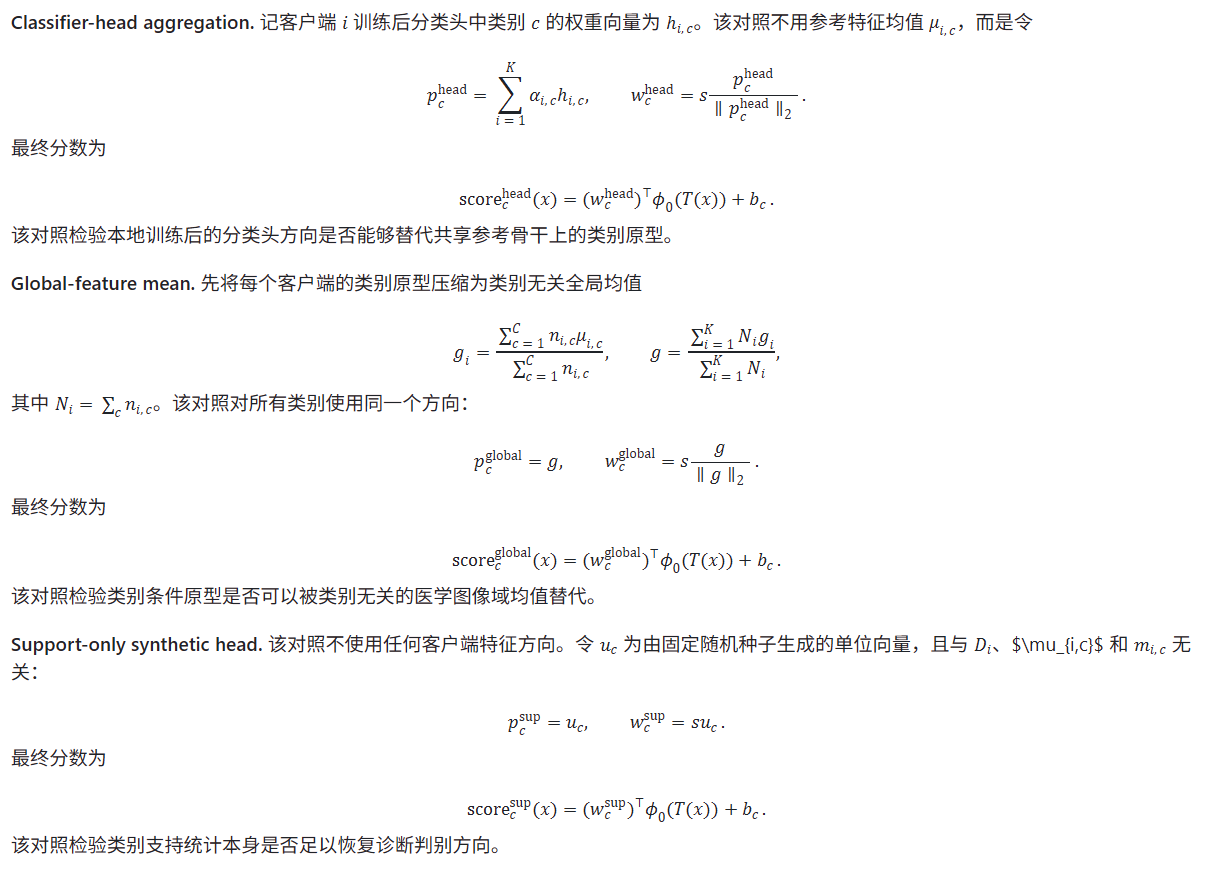
\includegraphics[width=\linewidth,keepaspectratio]{figures/image16.png}
\end{figure}

% --- DOCX block 102 ---
% Original image: image17.png
\begin{figure}[t]
\centering
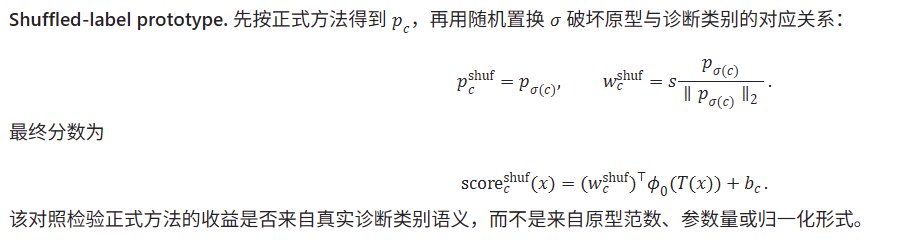
\includegraphics[width=\linewidth,keepaspectratio]{figures/image17.png}
\end{figure}

% --- DOCX block 103 ---
% Original: 类别统计信息
\subsubsection{Class Statistical Information}

% --- DOCX block 104 ---
% Original image: image18.png
\begin{figure}[t]
\centering
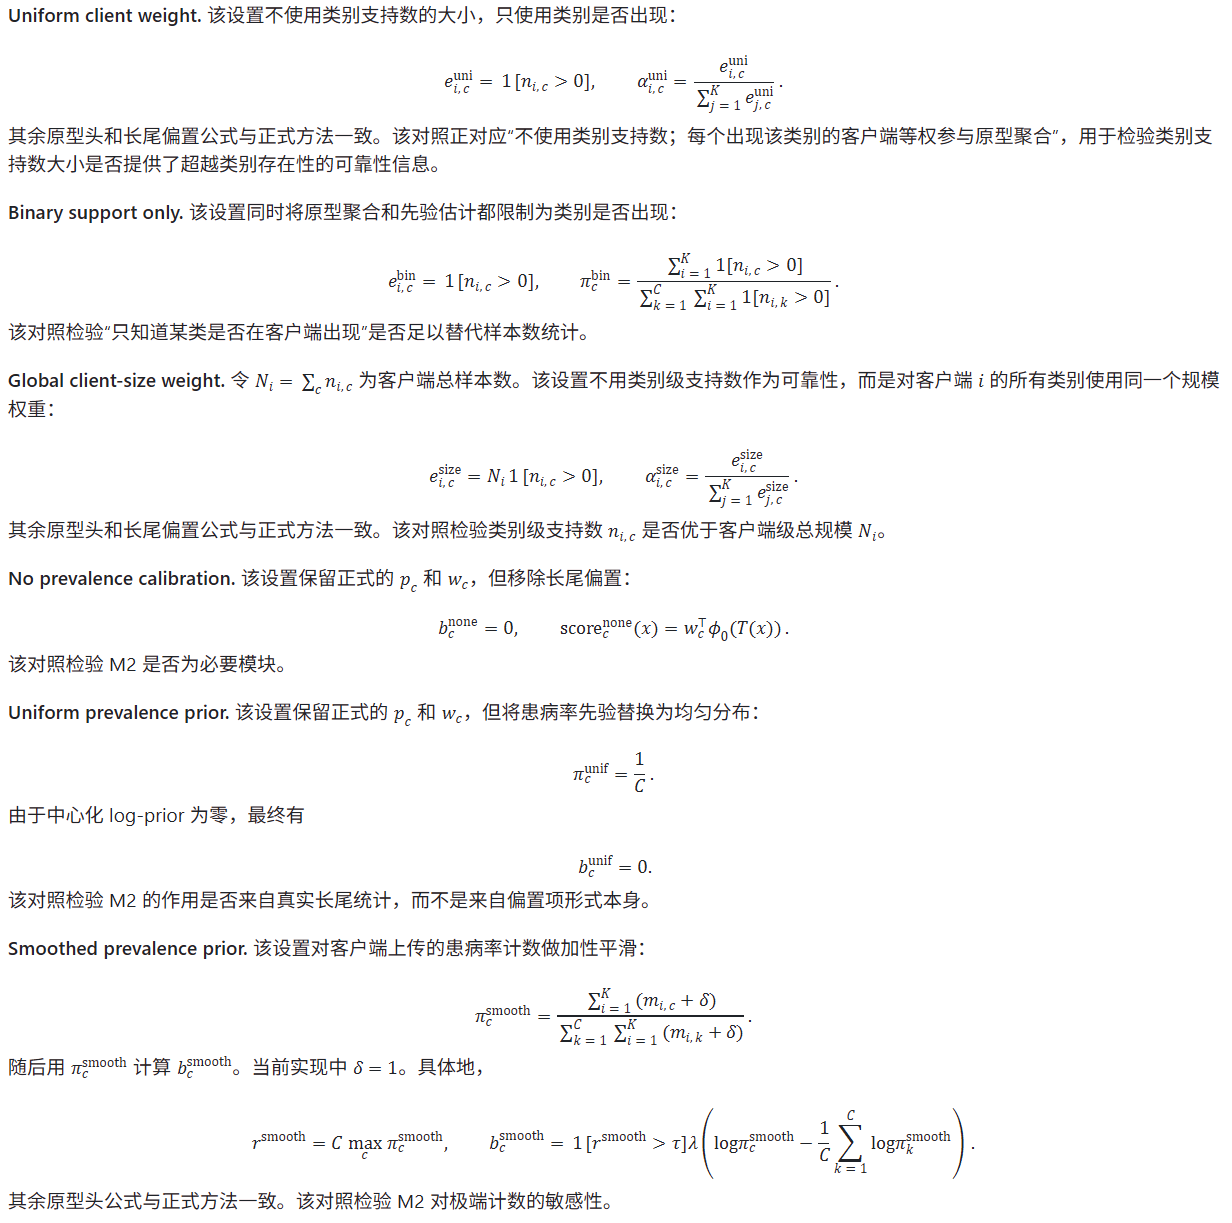
\includegraphics[width=\linewidth,keepaspectratio]{figures/image18.png}
\end{figure}

% --- DOCX block 105 ---
% Original: 注：No prevalence calibration到时候删掉，这是模块间消融
Note: No prevalence calibration should be deleted later; this is an inter-module ablation.


% --- DOCX block 106 ---
% Original table row: 设置 | Raw cells | Client-average mean Acc | Mean margin vs LAMP | Client-average >= LAMP
% Original table row: LAMP-Merge | 180 | 0.6209 | 0.0000 | 60/60
% Original table row: Classifier-head aggregation | 180 | 0.2579 | -0.3630 | 2/60
% Original table row: Global-feature mean | 180 | 0.2645 | -0.3564 | 9/60
% Original table row: Support-only synthetic head | 180 | 0.1137 | -0.5073 | 0/60
% Original table row: Shuffled-label prototype | 180 | 0.2002 | -0.4207 | 0/60
% Original table row: Uniform client weight | 180 | 0.5839 | -0.0370 | 3/60
% Original table row: Binary support only | 180 | 0.5517 | -0.0692 | 2/60
% Original table row: Global client-size weight | 180 | 0.5944 | -0.0266 | 5/60
% Original table row: No prevalence calibration | 180 | 0.5879 | -0.0330 | 24/60
% Original table row: Uniform prevalence prior | 180 | 0.5879 | -0.0330 | 24/60
% Original table row: Smoothed prevalence prior | 180 | 0.6209 | -0.0000 | 39/60
% Original table row: Smoothed prevalence prior | 180 | 0.6209 | -0.0000 | 39/6
\begin{table}[t]
\centering
\scriptsize
\setlength{\tabcolsep}{2pt}
\resizebox{\linewidth}{!}{%
\begin{tabular}{lcccc}
\toprule
Setting & Raw cells & Client-average mean Acc & Mean margin vs LAMP & Client-average >= LAMP \\
\midrule
LAMP-Merge & 180 & 0.6209 & 0.0000 & 60/60 \\
Classifier-head aggregation & 180 & 0.2579 & -0.3630 & 2/60 \\
Global-feature mean & 180 & 0.2645 & -0.3564 & 9/60 \\
Support-only synthetic head & 180 & 0.1137 & -0.5073 & 0/60 \\
Shuffled-label prototype & 180 & 0.2002 & -0.4207 & 0/60 \\
Uniform client weight & 180 & 0.5839 & -0.0370 & 3/60 \\
Binary support only & 180 & 0.5517 & -0.0692 & 2/60 \\
Global client-size weight & 180 & 0.5944 & -0.0266 & 5/60 \\
No prevalence calibration & 180 & 0.5879 & -0.0330 & 24/60 \\
Uniform prevalence prior & 180 & 0.5879 & -0.0330 & 24/60 \\
Smoothed prevalence prior & 180 & 0.6209 & -0.0000 & 39/60 \\
Smoothed prevalence prior & 180 & 0.6209 & -0.0000 & 39/6 \\
\bottomrule
\end{tabular}%
}
\end{table}

% --- DOCX block 107 ---
% Original image: image19.png
\begin{figure*}[t]
\centering
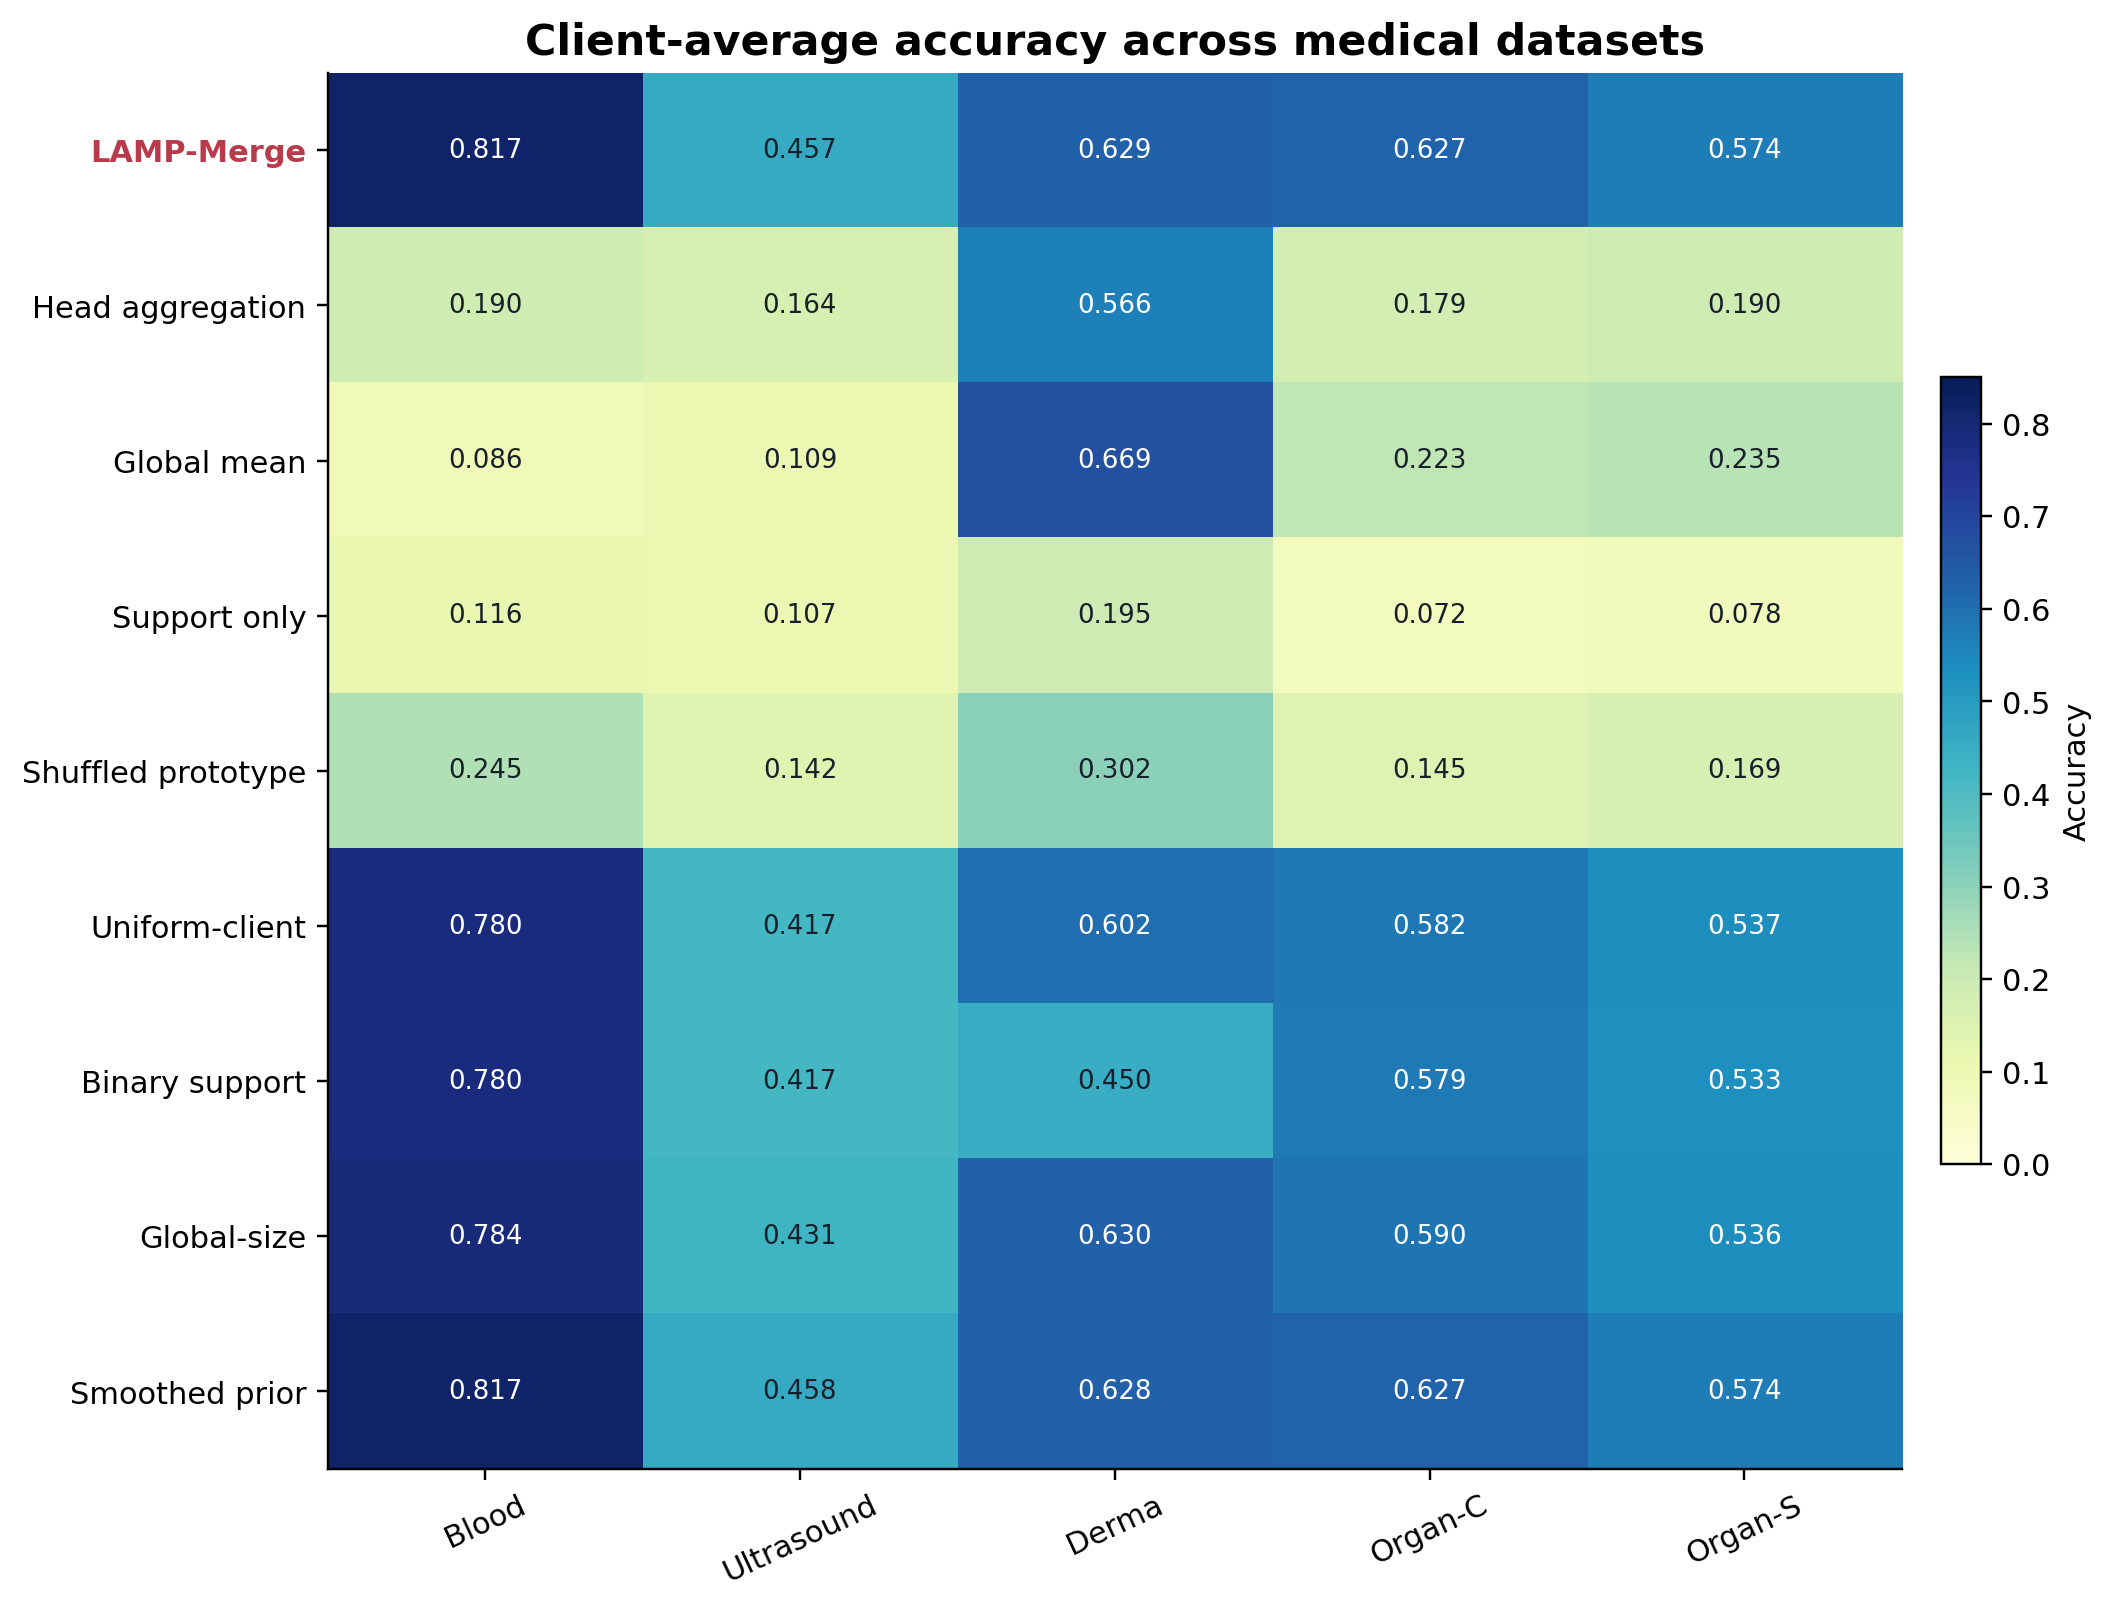
\includegraphics[width=\textwidth,keepaspectratio]{figures/image19.png}
\end{figure*}

% --- DOCX block 108 ---
% Original: 诊断原型替代项均显著低于正式方法，说明性能收益不能由额外分类头、随机方向或类别计数本身解释。No prevalence calibration 与 Uniform prevalence prior 均移除了有效长尾先验项，二者之间小于 5×10−5 的均值差异来自独立评估过程的浮点数值误差。加性平滑先验与正式方法仅相差 7.8×10−6，表明 M2 对轻微计数扰动稳定。
Diagnostic prototype alternatives are all significantly lower than the formal method, showing that the performance gain cannot be explained by an additional classifier head, random directions, or class counts alone. No prevalence calibration and Uniform prevalence prior both remove the effective long-tail prior term; their mean difference below $5\times10^{-5}$ comes from floating-point numerical differences in independent evaluation. The additive smoothed prior differs from the formal method by only $7.8\times10^{-6}$, showing that M2 is stable to mild count perturbations.


% --- DOCX block 109 ---
% Original: 模块间消融
\subsection{Inter-module Ablation}

% --- DOCX block 110 ---
% Original: 模块间消融采用正式主表口径，覆盖 5 个数据集、5 个 backbone、3 个客户端数量与 3 个 Dirichlet β，共 225 个 raw cells 和 75 个 client-average cells。该表直接比较完整 LAMP-Merge、仅保留诊断原型重建的 M1 only、将 M2 附加到普通平均模型的 avg+M2，以及普通参数平均 avg。
The inter-module ablation follows the formal main-table protocol, covering 5 datasets, 5 backbones, 3 client counts, and 3 Dirichlet $\beta$ values, for a total of 225 raw cells and 75 client-average cells. This table directly compares complete LAMP-Merge, M1 only with diagnostic prototype reconstruction retained, avg+M2 which attaches M2 to ordinary averaging, and ordinary parameter averaging avg.


% --- DOCX block 111 ---
% Original table row: 设置 | Client-average cells | Client-average mean Acc | Best/tied cells | >= avg cells | Mean margin vs avg
% Original table row: LAMP-Merge | 75 | 0.5618 | 51/75 | 71/75 | +0.3345
% Original table row: M1 only | 75 | 0.5362 | 46/75 | 66/75 | +0.3089
% Original table row: avg+M2 | 75 | 0.2198 | 4/75 | 43/75 | -0.0075
% Original table row: avg | 75 | 0.2273 | 2/75 | 75/75 | 0.0000
\begin{table}[t]
\centering
\scriptsize
\setlength{\tabcolsep}{2pt}
\resizebox{\linewidth}{!}{%
\begin{tabular}{lccccc}
\toprule
Setting & Client-average cells & Client-average mean Acc & Best/tied cells & >= avg cells & Mean margin vs avg \\
\midrule
LAMP-Merge & 75 & 0.5618 & 51/75 & 71/75 & +0.3345 \\
M1 only & 75 & 0.5362 & 46/75 & 66/75 & +0.3089 \\
avg+M2 & 75 & 0.2198 & 4/75 & 43/75 & -0.0075 \\
avg & 75 & 0.2273 & 2/75 & 75/75 & 0.0000 \\
\bottomrule
\end{tabular}%
}
\end{table}

% --- DOCX block 112 ---
% Original: 数据集级模块间消融如下：
The dataset-level inter-module ablation is as follows:


% --- DOCX block 113 ---
% Original table row: Dataset | Cells | LAMP-Merge | M1 only | avg+M2 | avg | LAMP best/tied
% Original table row: bloodmnist_224 | 15 | 0.7156 | 0.7155 | 0.1726 | 0.1699 | 12/15
% Original table row: chaoshengmnist_224 | 15 | 0.4040 | 0.4040 | 0.1551 | 0.1516 | 15/15
% Original table row: dermamnist_224 | 15 | 0.6257 | 0.4975 | 0.4913 | 0.5304 | 12/15
% Original table row: organcmnist_224 | 15 | 0.5543 | 0.5543 | 0.1331 | 0.1358 | 6/15
% Original table row: organsmnist_224 | 15 | 0.5096 | 0.5096 | 0.1469 | 0.1488 | 6/15
\begin{table}[t]
\centering
\scriptsize
\setlength{\tabcolsep}{2pt}
\resizebox{\linewidth}{!}{%
\begin{tabular}{lcccccc}
\toprule
Dataset & Cells & LAMP-Merge & M1 only & avg+M2 & avg & LAMP best/tied \\
\midrule
bloodmnist\_224 & 15 & 0.7156 & 0.7155 & 0.1726 & 0.1699 & 12/15 \\
chaoshengmnist\_224 & 15 & 0.4040 & 0.4040 & 0.1551 & 0.1516 & 15/15 \\
dermamnist\_224 & 15 & 0.6257 & 0.4975 & 0.4913 & 0.5304 & 12/15 \\
organcmnist\_224 & 15 & 0.5543 & 0.5543 & 0.1331 & 0.1358 & 6/15 \\
organsmnist\_224 & 15 & 0.5096 & 0.5096 & 0.1469 & 0.1488 & 6/15 \\
\bottomrule
\end{tabular}%
}
\end{table}

% --- DOCX block 114 ---
% Original: 超参数分析
\section{Hyperparameter Analysis}

% --- DOCX block 115 ---
% Original: 超参数分析汇总每个内部因素的取值范围、最佳点、最差点和波动幅度，用于说明正式取值不是依赖单点偶然收益。
The hyperparameter analysis summarizes the value range, best point, worst point, and fluctuation amplitude of each internal factor, showing that the formal setting does not rely on an accidental single-point gain.


% --- DOCX block 116 ---
% Original: 全量结果表明，LAMP-Merge 对两个超参数均具有稳定平台，而不是依赖单点调参。对于 M1，s=20 取得最高 client-average mean Accuracy 0.6209；在 s∈[12,22] 内，平均 Accuracy 始终保持在 0.6204 至 0.6209 之间，说明诊断原型头只需要适度 logit 尺度即可稳定工作。对于 M2，λ=5 取得最高 client-average mean Accuracy 0.6209；在 λ∈[4,8] 内，平均 Accuracy 始终保持在 0.6198 至 0.6209 之间，说明长尾校准的收益来自有界医学患病率先验，而不是无界追随多数类。
Full-scope results show that LAMP-Merge has a stable plateau for both hyperparameters, rather than relying on single-point tuning. For M1, $s=20$ obtains the highest client-average mean Accuracy of 0.6209; within $s\in[12,22]$, the mean Accuracy remains between 0.6204 and 0.6209, indicating that the diagnostic prototype head only needs a moderate logit scale to work stably. For M2, $\lambda=5$ obtains the highest client-average mean Accuracy of 0.6209; within $\lambda\in[4,8]$, the mean Accuracy remains between 0.6198 and 0.6209, indicating that the benefit of long-tail calibration comes from a bounded medical prevalence prior rather than unboundedly following the majority class.

% Original image: image20.png
\begin{figure*}[t]
\centering
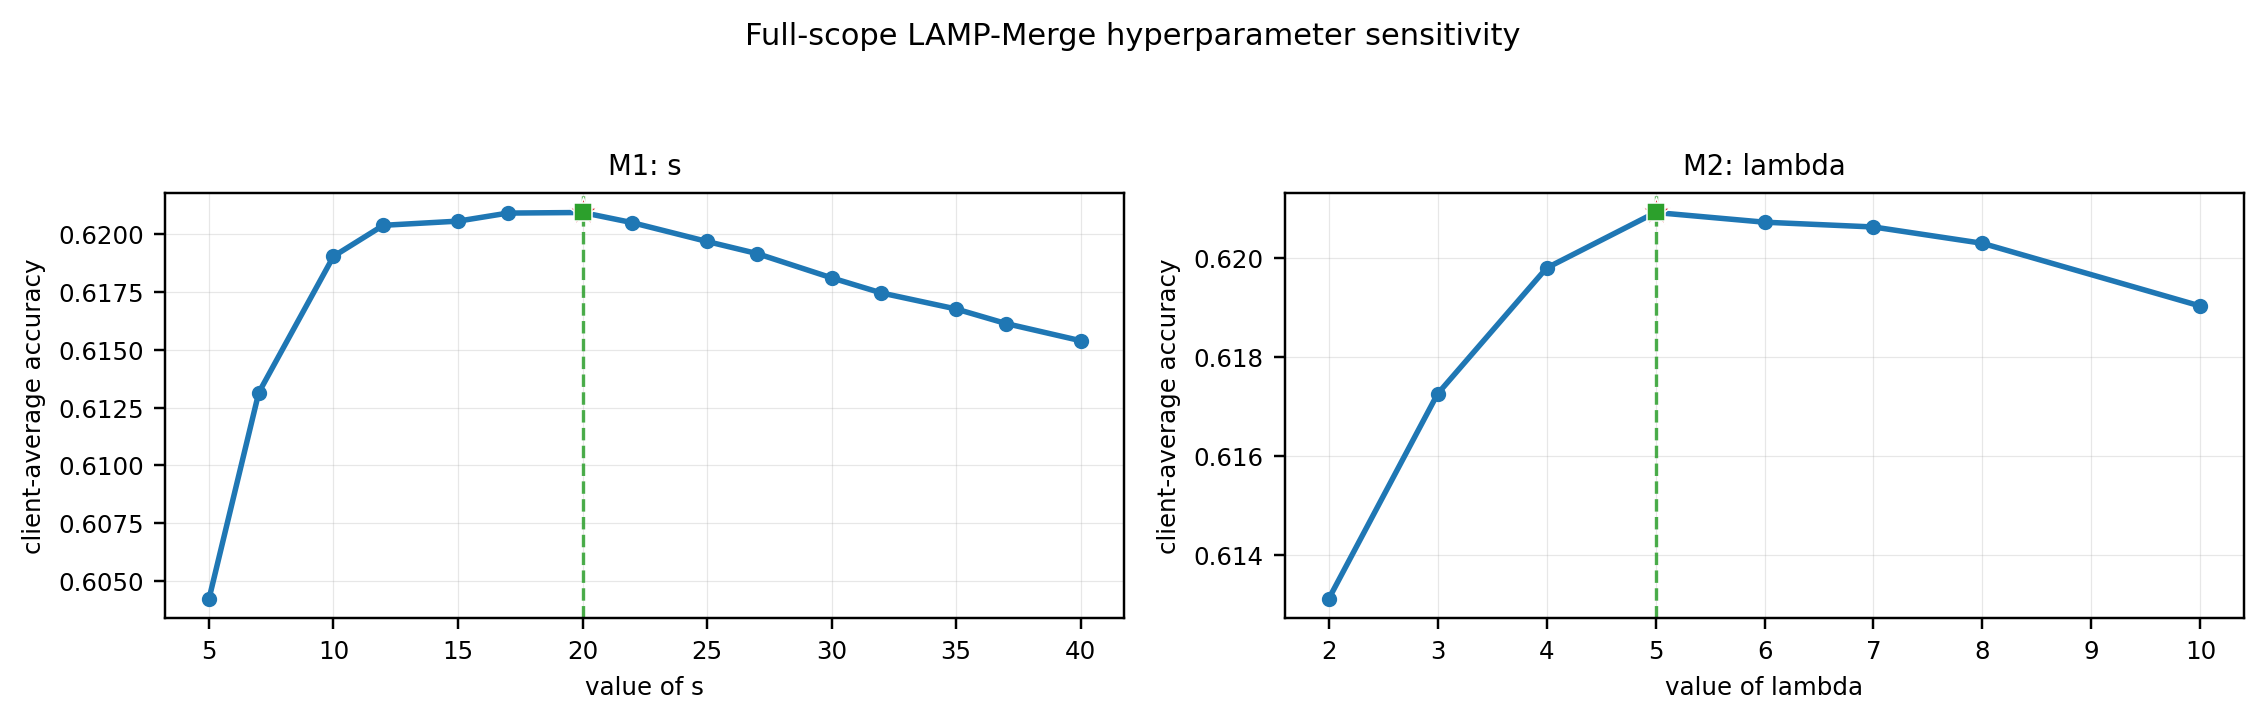
\includegraphics[width=\textwidth,keepaspectratio]{figures/image20.png}
\end{figure*}

% --- DOCX block 117 ---
% Original: 新指标诊断实验
\section{Additional Metric Diagnostic Experiment}

% --- DOCX block 118 ---
% Original: 为排除 LAMP-Merge 仅利用多数类 accuracy 的可能性，我们额外构造预测分布诊断实验。该实验覆盖 5 个正式医学数据集，每个数据集使用 4 个 backbone（resnet、convnext、vit_t、swin_tiny）固定clients=3, beta=0.01, seed=42。统计对象包括 individual clients 的聚合行、通用模型融合 baseline，以及 LAMP-Merge。
To rule out the possibility that LAMP-Merge only exploits majority-class Accuracy, we additionally construct a prediction-distribution diagnostic experiment. This experiment covers 5 formal medical datasets, each using 4 backbones (resnet, convnext, vit\_t, and swin\_tiny) with clients=3, beta=0.01, and seed=42. The measured objects include aggregate rows for individual clients, general model-merging baselines, and LAMP-Merge.


% --- DOCX block 119 ---
% Original: 除 Accuracy 外，该实验报告以下新指标：
In addition to Accuracy, this experiment reports the following new metrics:


% --- DOCX block 120 ---
% Original image: image21.png
\begin{center}
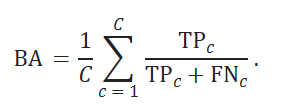
\includegraphics[width=0.62\linewidth,keepaspectratio]{figures/image21.png}
\end{center}

% --- DOCX block 121 ---
% Original: 其中 BA 是 balanced accuracy，即 macro recall，用于衡量各诊断类别是否同时被召回。设 q(c) 表示模型在测试集上预测为类别 c 的比例，p(c) 表示测试集真实类别比例，则预测坍缩强度与预测分布偏差定义为：
Here, BA is balanced accuracy, i.e., macro recall, used to measure whether all diagnostic classes are recalled. Let $q(c)$ denote the proportion of predictions assigned to class $c$ on the test set, and let $p(c)$ denote the true class proportion in the test set. Then prediction-collapse strength and prediction-distribution deviation are defined as:

% Original image: image22.png
\begin{center}
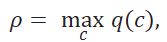
\includegraphics[width=0.62\linewidth,keepaspectratio]{figures/image22.png}
\end{center}

% --- DOCX block 122 ---
% Original image: image23.png
\begin{center}
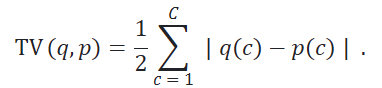
\includegraphics[width=0.62\linewidth,keepaspectratio]{figures/image23.png}
\end{center}

% --- DOCX block 123 ---
% Original: ρ 越接近 1，模型越接近单类预测器；TV(q,p) 越小，预测类别分布越接近真实诊断分布。有效预测类别数定义为：
The closer $\rho$ is to 1, the closer the model is to a single-class predictor; the smaller $TV(q,p)$ is, the closer the predicted class distribution is to the true diagnostic distribution. The effective number of predicted classes is defined as:


% --- DOCX block 124 ---
% Original image: image24.png
\begin{center}
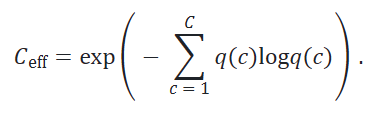
\includegraphics[width=0.62\linewidth,keepaspectratio]{figures/image24.png}
\end{center}

% --- DOCX block 125 ---
% Original: 该指标越大，表示模型实际使用的诊断类别越多。若一个方法仅在多数类上坍缩，则通常会表现为 Accuracy 较高但 BA、Macro F1 和 Ceff 较低，同时 ρ 和 TV 较高。
A larger value indicates that the model actually uses more diagnostic classes. If a method only collapses to the majority class, it usually shows high Accuracy but low BA, Macro F1, and $C_{\mathrm{eff}}$, while $\rho$ and TV are high.


% --- DOCX block 126 ---
% Original table row: 设置 | BA ↑ | Macro-F1 ↑ | ρ ↓ | Ceff ↑ | Pred-True TV ↓
% Original table row: LAMP-Merge | 0.5370 | 0.5238 | 0.3122 | 7.1322 | 0.1262
% Original table row: Classifier-head aggregation | 0.1420 | 0.0932 | 0.6679 | 2.7812 | 0.5386
% Original table row: Global-feature mean | 0.1149 | 0.0448 | 0.9996 | 1.0015 | 0.7381
% Original table row: Support-only synthetic head | 0.1147 | 0.0590 | 0.6099 | 3.3330 | 0.6287
% Original table row: Shuffled-label prototype | 0.1425 | 0.1316 | 0.2564 | 7.4060 | 0.2630
% Original table row: Uniform client weight | 0.5001 | 0.4821 | 0.3232 | 6.9106 | 0.1628
% Original table row: Binary support only | 0.5294 | 0.4901 | 0.2496 | 7.7057 | 0.1840
% Original table row: Global client-size weight | 0.5028 | 0.4852 | 0.3293 | 6.8625 | 0.1543
% Original table row: Smoothed prevalence prior | 0.5371 | 0.5238 | 0.3120 | 7.1357 | 0.1261
\begin{table}[t]
\centering
\scriptsize
\setlength{\tabcolsep}{2pt}
\resizebox{\linewidth}{!}{%
\begin{tabular}{lccccc}
\toprule
Setting & BA $\uparrow$ & Macro-F1 $\uparrow$ & $\rho \downarrow$ & $C_{\mathrm{eff}} \uparrow$ & Pred-True TV $\downarrow$ \\
\midrule
LAMP-Merge & 0.5370 & 0.5238 & 0.3122 & 7.1322 & 0.1262 \\
Classifier-head aggregation & 0.1420 & 0.0932 & 0.6679 & 2.7812 & 0.5386 \\
Global-feature mean & 0.1149 & 0.0448 & 0.9996 & 1.0015 & 0.7381 \\
Support-only synthetic head & 0.1147 & 0.0590 & 0.6099 & 3.3330 & 0.6287 \\
Shuffled-label prototype & 0.1425 & 0.1316 & 0.2564 & 7.4060 & 0.2630 \\
Uniform client weight & 0.5001 & 0.4821 & 0.3232 & 6.9106 & 0.1628 \\
Binary support only & 0.5294 & 0.4901 & 0.2496 & 7.7057 & 0.1840 \\
Global client-size weight & 0.5028 & 0.4852 & 0.3293 & 6.8625 & 0.1543 \\
Smoothed prevalence prior & 0.5371 & 0.5238 & 0.3120 & 7.1357 & 0.1261 \\
\bottomrule
\end{tabular}%
}
\end{table}

% --- DOCX block 127 ---
% Original image: image25.png
\begin{figure*}[t]
\centering
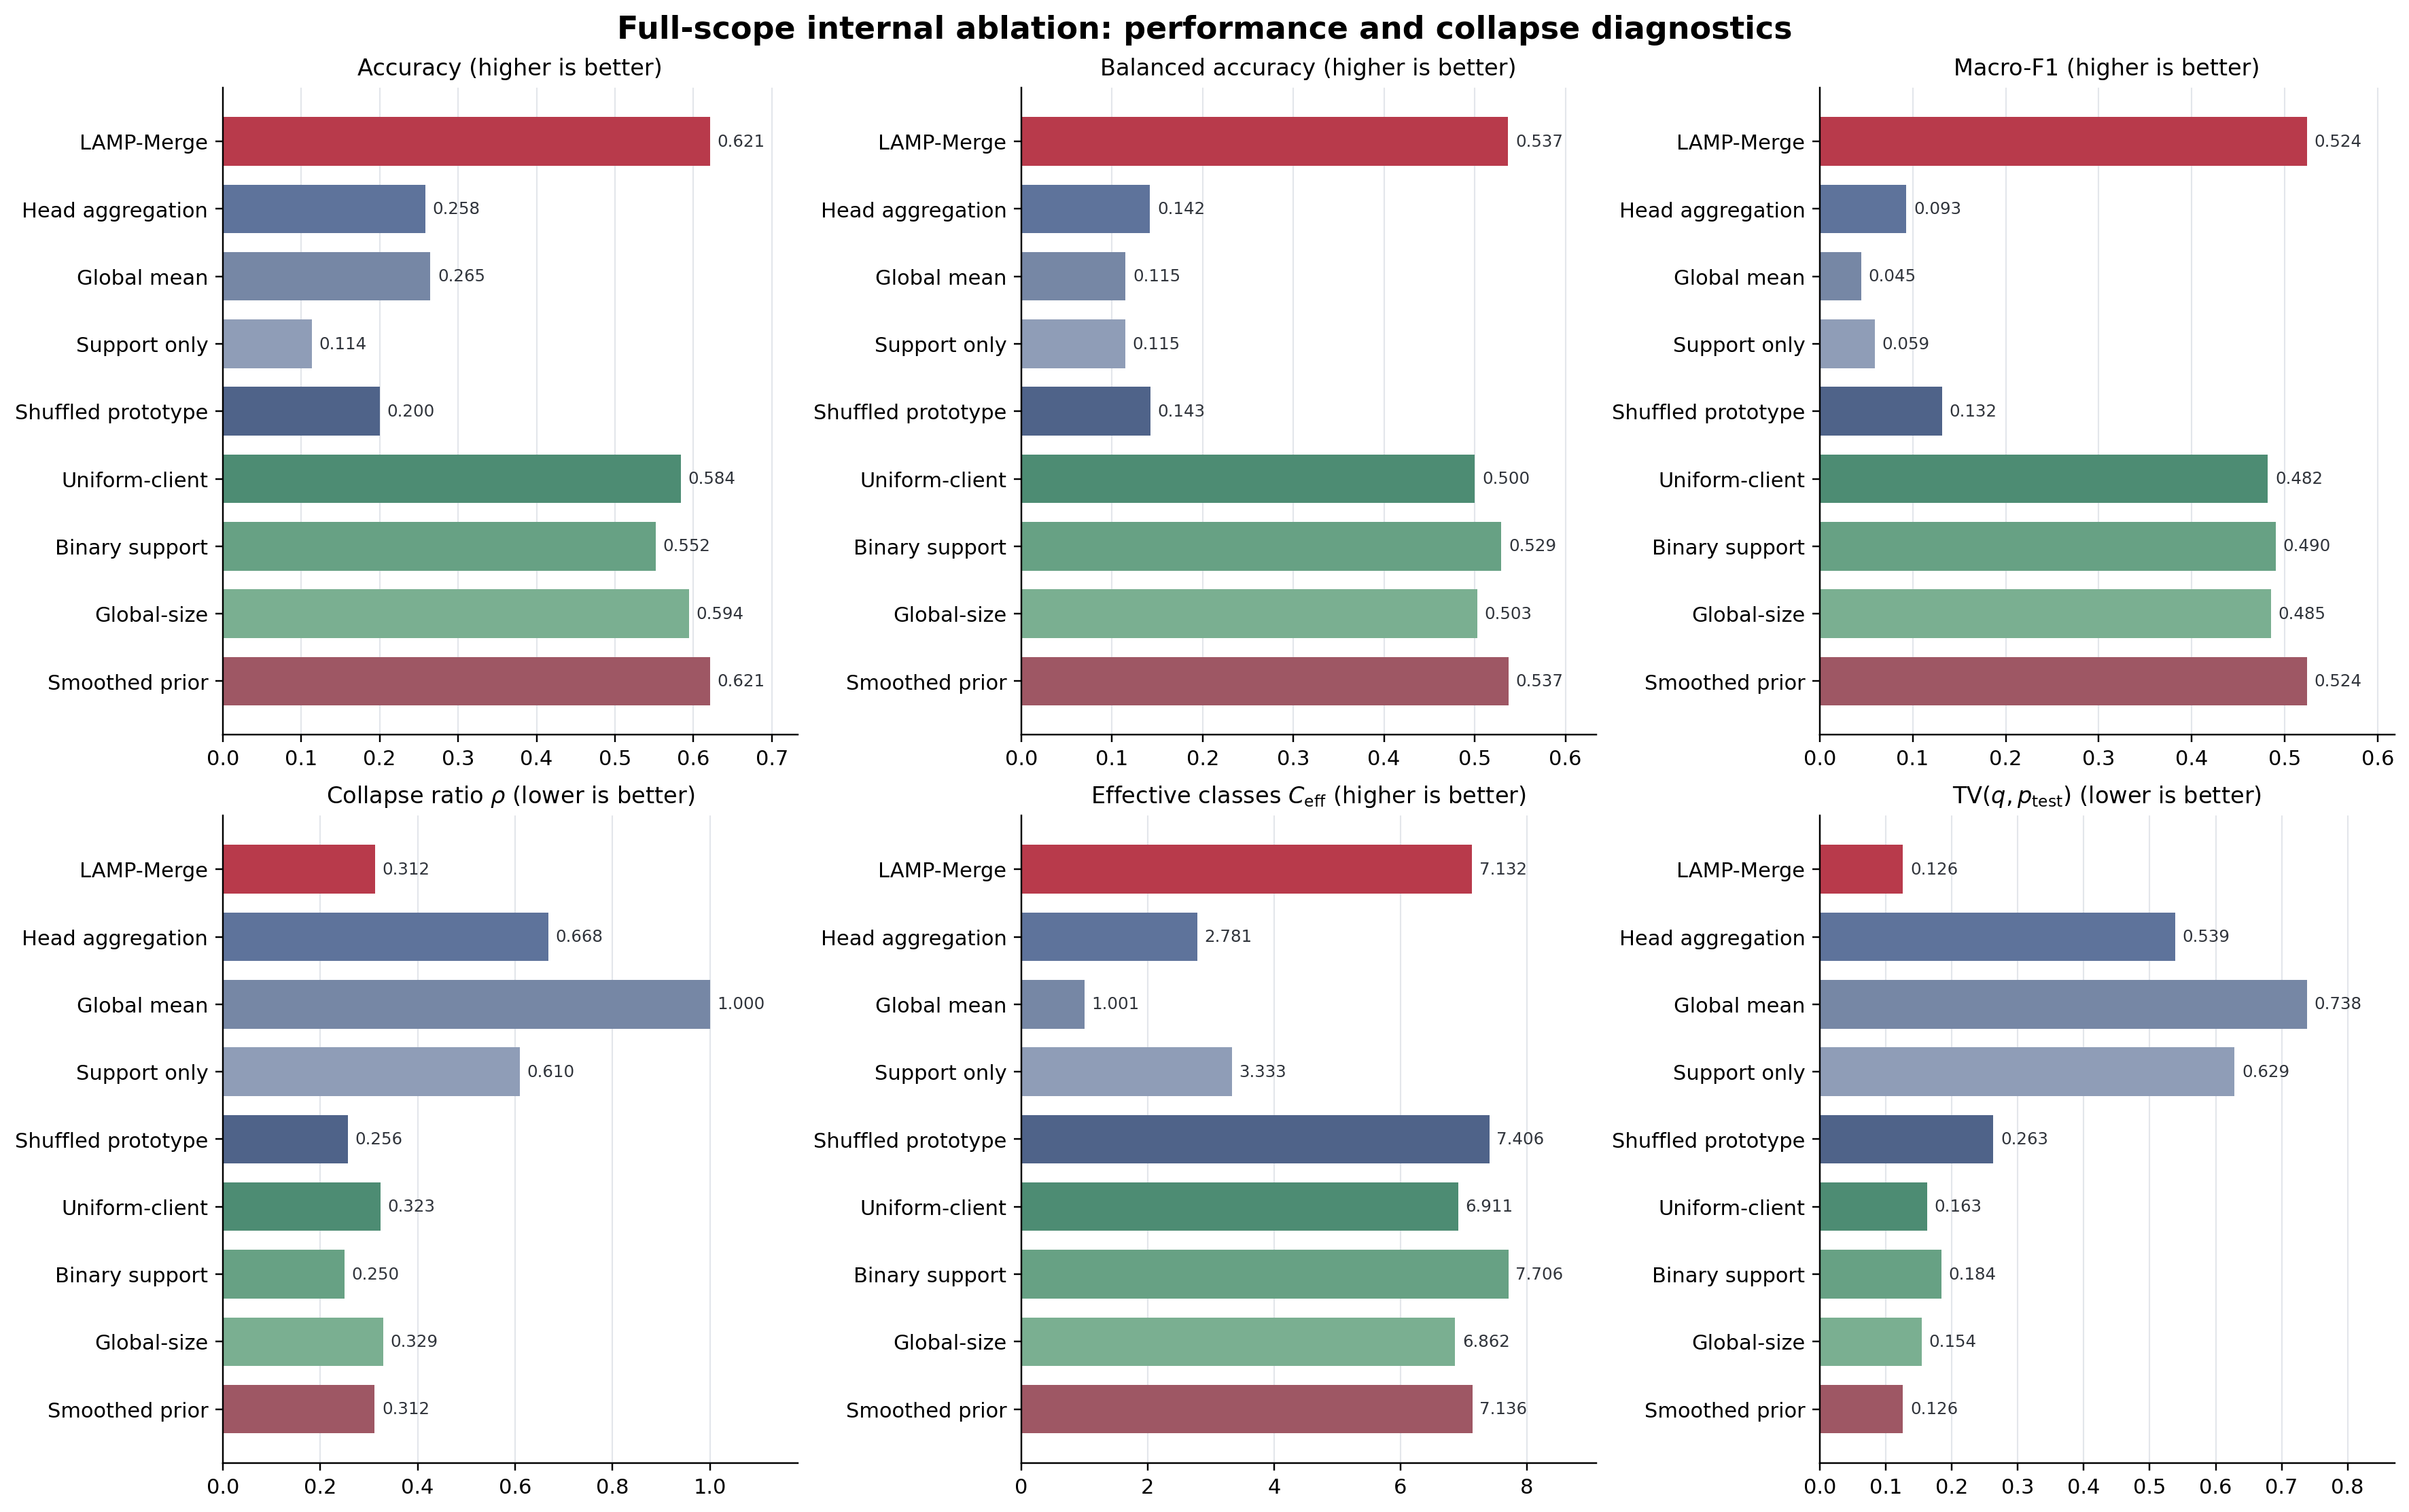
\includegraphics[width=\textwidth,keepaspectratio]{figures/image25.png}
\end{figure*}

% --- DOCX block 128 ---
% Original: M1-only 具有更高的 BA、Macro-F1 和 Ceff，说明诊断原型直接恢复了多类别判别结构。LAMP-Merge 的总体 Accuracy 更高、Pred-True TV 更低，说明 M2 将预测分布校准到真实医学患病率。二者并不矛盾：M1 优化类别均衡判别，M2 在强长尾条件下优化与真实测试分布一致的总体风险。
M1-only has higher BA, Macro-F1, and $C_{\mathrm{eff}}$, indicating that diagnostic prototypes directly restore multi-class discrimination. LAMP-Merge has higher overall Accuracy and lower Pred-True TV, indicating that M2 calibrates the prediction distribution to the real medical prevalence. These are not contradictory: M1 optimizes class-balanced discrimination, while M2 optimizes overall risk consistent with the true test distribution under strong long-tail conditions.


% --- DOCX block 129 ---
% Original:   按数据集结果：
Dataset-level results:


% --- DOCX block 130 ---
% Original table row: Dataset | Setting | BA | Macro-F1 | ρ | Ceff | Pred-True TV
% Original table row: bloodmnist_224 | Best generic (iso_c) | 0.1730 | 0.0860 | 0.8020 | 1.8145 | 0.7348
% Original table row: bloodmnist_224 | LAMP-Merge | 0.8058 | 0.8011 | 0.1958 | 7.4795 | 0.0394
% Original table row: chaoshengmnist_224 | Best generic (fisher) | 0.1595 | 0.0753 | 0.8603 | 1.5414 | 0.7679
% Original table row: chaoshengmnist_224 | LAMP-Merge | 0.4481 | 0.4329 | 0.2042 | 7.4419 | 0.1538
% Original table row: dermamnist_224 | Best generic (free_merge) | 0.1504 | 0.0997 | 0.9522 | 1.1641 | 0.4606
% Original table row: dermamnist_224 | LAMP-Merge | 0.3242 | 0.2773 | 0.6995 | 2.9585 | 0.1737
% Original table row: organcmnist_224 | Best generic (robustmerge) | 0.1194 | 0.0494 | 0.8174 | 1.7291 | 0.7870
% Original table row: organcmnist_224 | LAMP-Merge | 0.5951 | 0.5915 | 0.2115 | 9.4702 | 0.1250
% Original table row: organsmnist_224 | Best generic (robustmerge) | 0.1193 | 0.0538 | 0.7888 | 1.9973 | 0.7385
% Original table row: organsmnist_224 | LAMP-Merge | 0.5118 | 0.5162 | 0.2499 | 8.3109 | 0.1389
\begin{table}[t]
\centering
\scriptsize
\setlength{\tabcolsep}{2pt}
\resizebox{\linewidth}{!}{%
\begin{tabular}{lcccccc}
\toprule
Dataset & Setting & BA & Macro-F1 & ρ & Ceff & Pred-True TV \\
\midrule
bloodmnist\_224 & Best generic (iso\_c) & 0.1730 & 0.0860 & 0.8020 & 1.8145 & 0.7348 \\
bloodmnist\_224 & LAMP-Merge & 0.8058 & 0.8011 & 0.1958 & 7.4795 & 0.0394 \\
chaoshengmnist\_224 & Best generic (fisher) & 0.1595 & 0.0753 & 0.8603 & 1.5414 & 0.7679 \\
chaoshengmnist\_224 & LAMP-Merge & 0.4481 & 0.4329 & 0.2042 & 7.4419 & 0.1538 \\
dermamnist\_224 & Best generic (free\_merge) & 0.1504 & 0.0997 & 0.9522 & 1.1641 & 0.4606 \\
dermamnist\_224 & LAMP-Merge & 0.3242 & 0.2773 & 0.6995 & 2.9585 & 0.1737 \\
organcmnist\_224 & Best generic (robustmerge) & 0.1194 & 0.0494 & 0.8174 & 1.7291 & 0.7870 \\
organcmnist\_224 & LAMP-Merge & 0.5951 & 0.5915 & 0.2115 & 9.4702 & 0.1250 \\
organsmnist\_224 & Best generic (robustmerge) & 0.1193 & 0.0538 & 0.7888 & 1.9973 & 0.7385 \\
organsmnist\_224 & LAMP-Merge & 0.5118 & 0.5162 & 0.2499 & 8.3109 & 0.1389 \\
\bottomrule
\end{tabular}%
}
\end{table}

% --- DOCX block 131 ---
% Original: best generic表示在每个数据集上按 full-scope mean Accuracy 选出的最强固定通用融合基线，仅用于分析，不参与 LAMP-Merge 的模型选择。
best generic denotes the strongest fixed general merging baseline selected by full-scope mean Accuracy on each dataset. It is used only for analysis and does not participate in LAMP-Merge model selection.


% --- DOCX block 132 ---
% Original image: image26.png
\begin{figure*}[t]
\centering
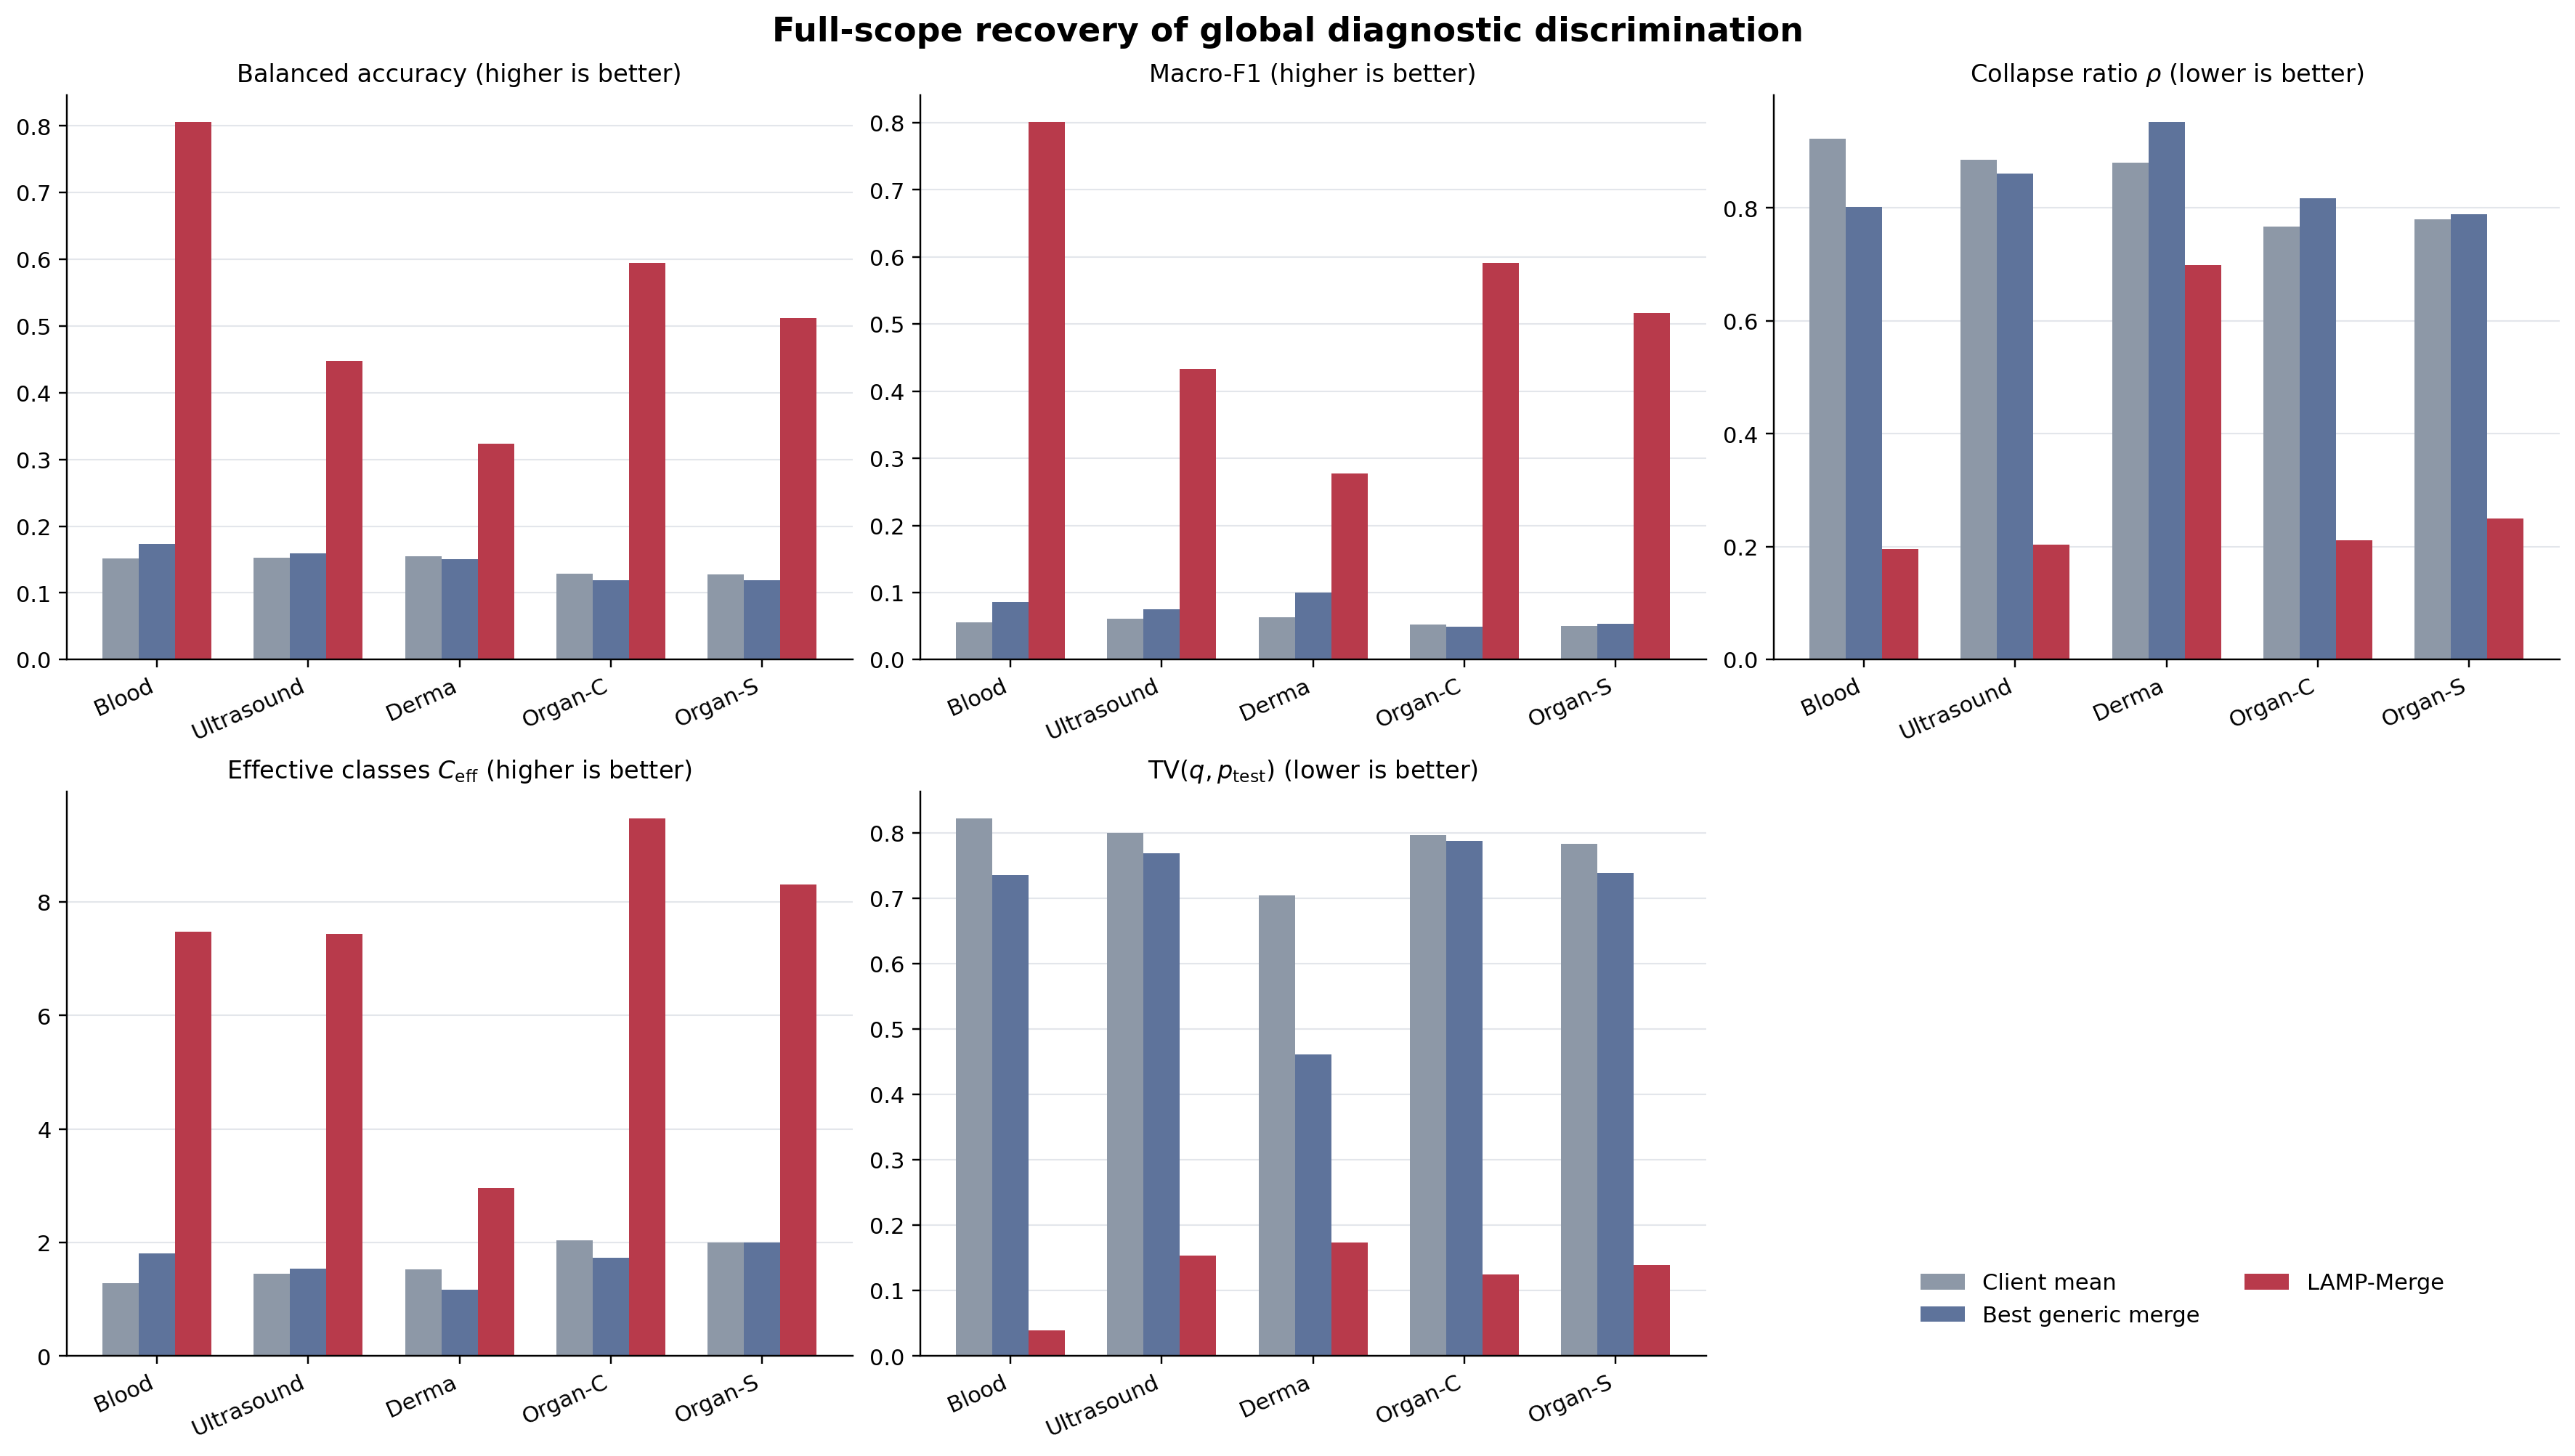
\includegraphics[width=\textwidth,keepaspectratio]{figures/image26.png}
\end{figure*}

% --- DOCX block 133 ---
% Original: 预测分布可视化
\subsection{Prediction Distribution Visualization}

% --- DOCX block 134 ---
% Original: 下图在 Derma 的 36 个 full-scope cases 上聚合预测类别比例。测试集类别 5 的真实比例为 0.67；M1-only 的预测比例为 0.38，LAMP-Merge 经 M2 校准后为 0.70。相比之下，最强通用基线free_merge的坍缩强度为 0.9522。由此可见，M2 不是无约束地追随多数类，而是将 M1 的均衡预测分布校准到客户端上传计数所估计的真实长尾先验。
The following figure aggregates predicted class proportions over 36 full-scope cases on Derma. The true proportion of test-set class 5 is 0.67; the predicted proportion of M1-only is 0.38, while LAMP-Merge reaches 0.70 after M2 calibration. In contrast, the collapse strength of the strongest general baseline free\_merge is 0.9522. Thus, M2 does not follow the majority class without constraint, but calibrates the balanced prediction distribution of M1 to the true long-tail prior estimated from client-uploaded counts.


% --- DOCX block 135 ---
% Original: 其余数据集如下：
The remaining datasets are as follows:

% Original image: image27.png
\begin{figure}[t]
\centering
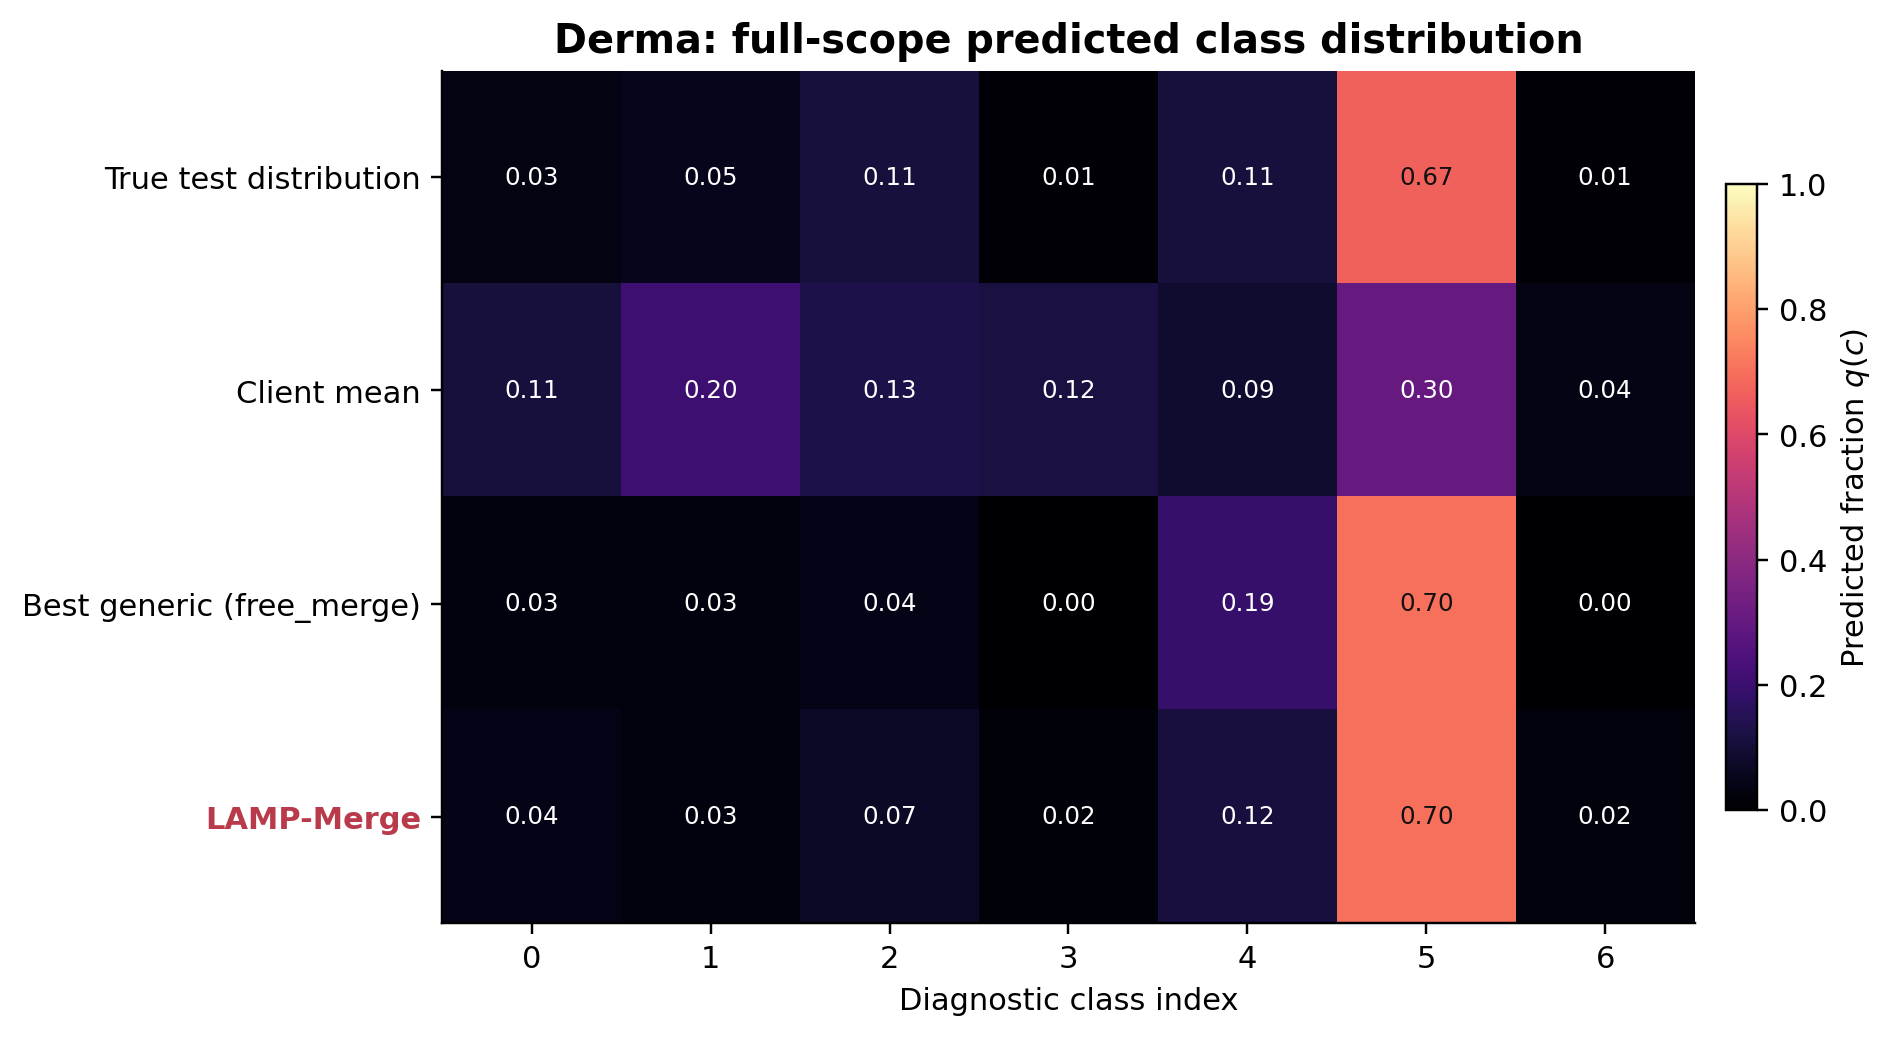
\includegraphics[width=\linewidth,keepaspectratio]{figures/image27.png}
\end{figure}

% --- DOCX block 136 ---
% Original image: image28.png
\begin{figure}[t]
\centering
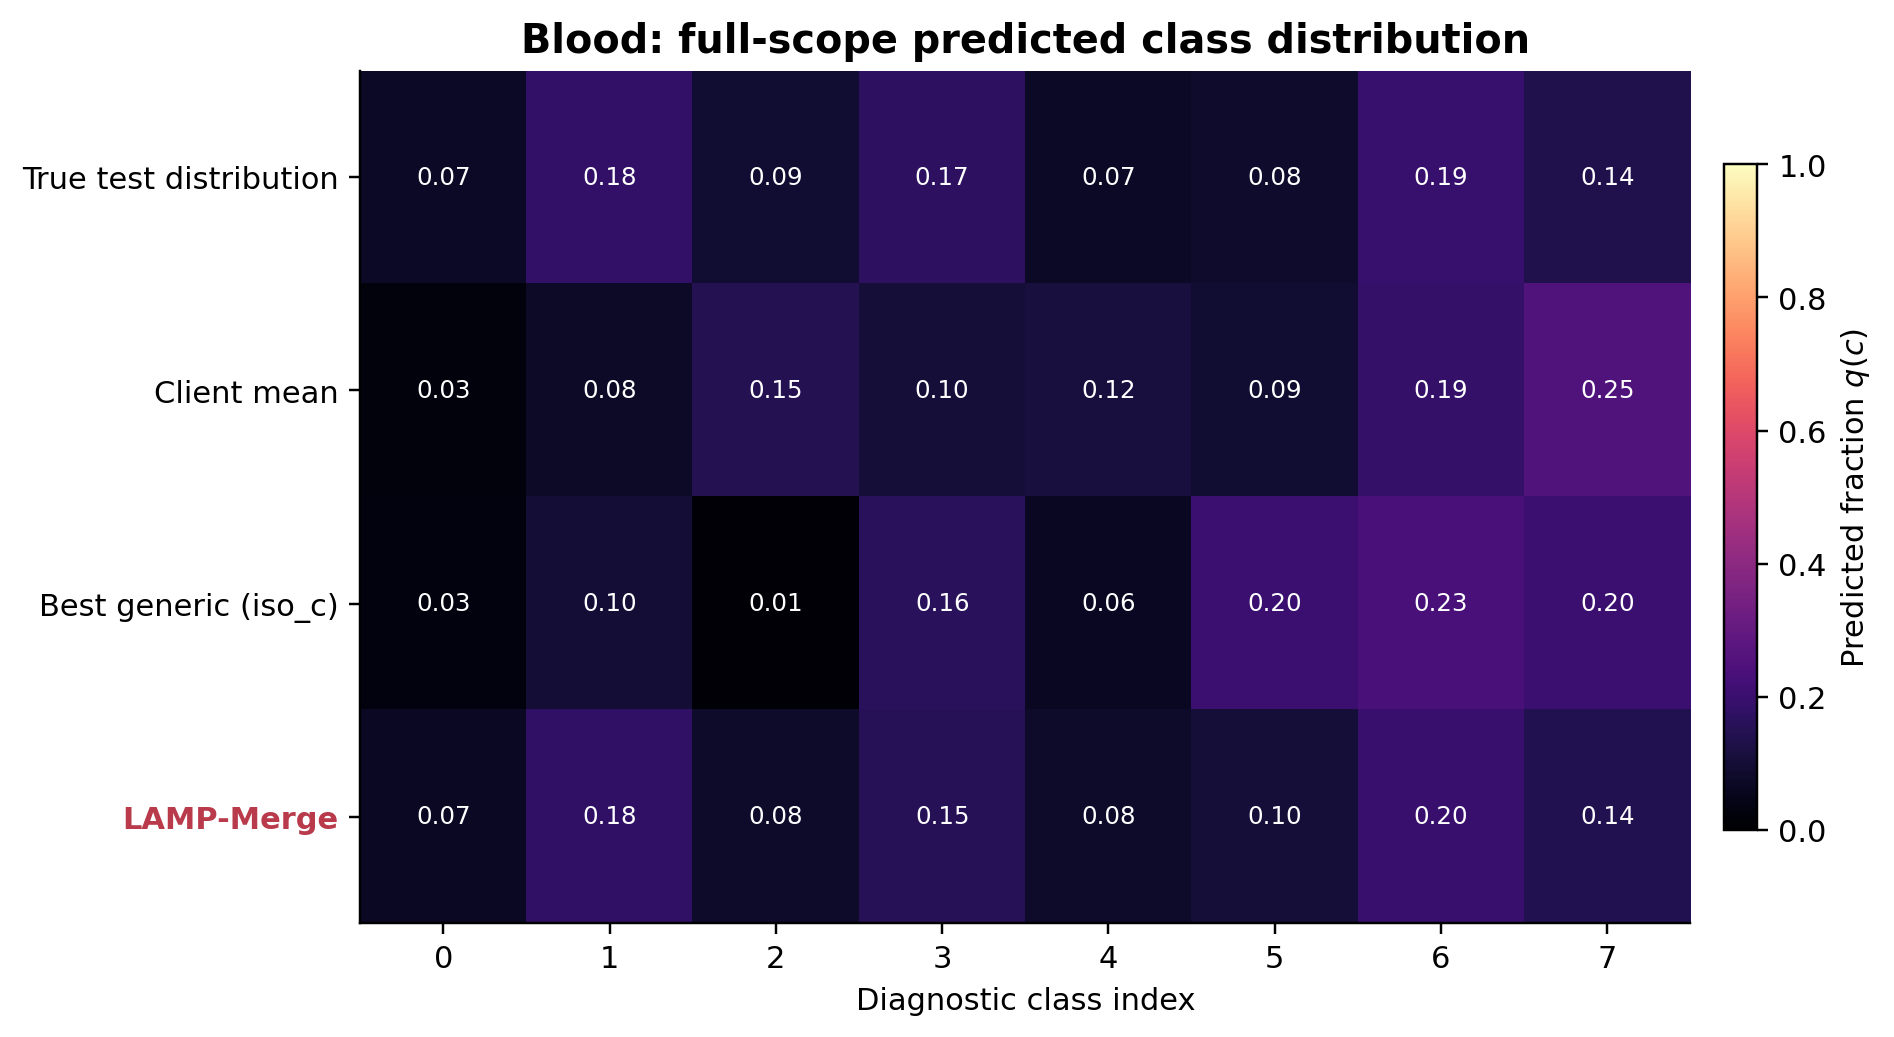
\includegraphics[width=\linewidth,keepaspectratio]{figures/image28.png}
\end{figure}

% --- DOCX block 137 ---
% Original image: image29.png
\begin{figure}[t]
\centering
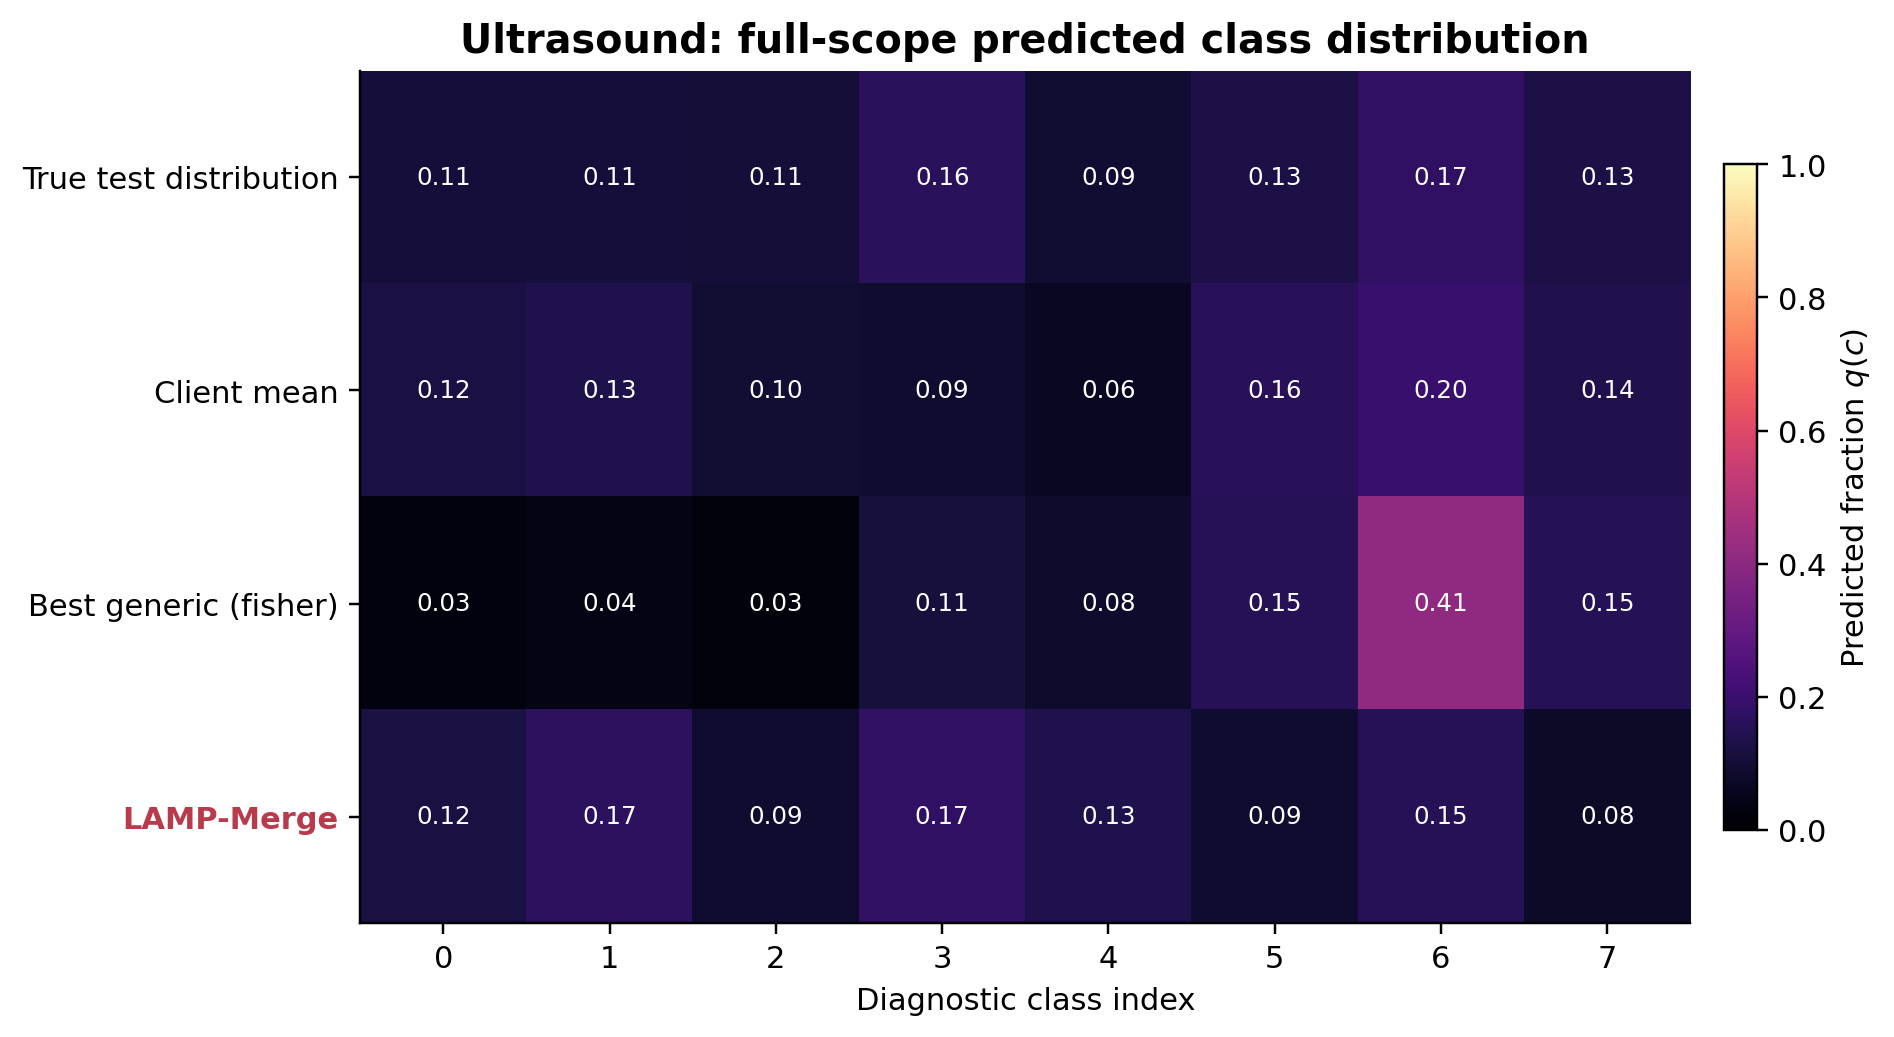
\includegraphics[width=\linewidth,keepaspectratio]{figures/image29.png}
\end{figure}
% Original image: image30.png
\begin{figure}[t]
\centering
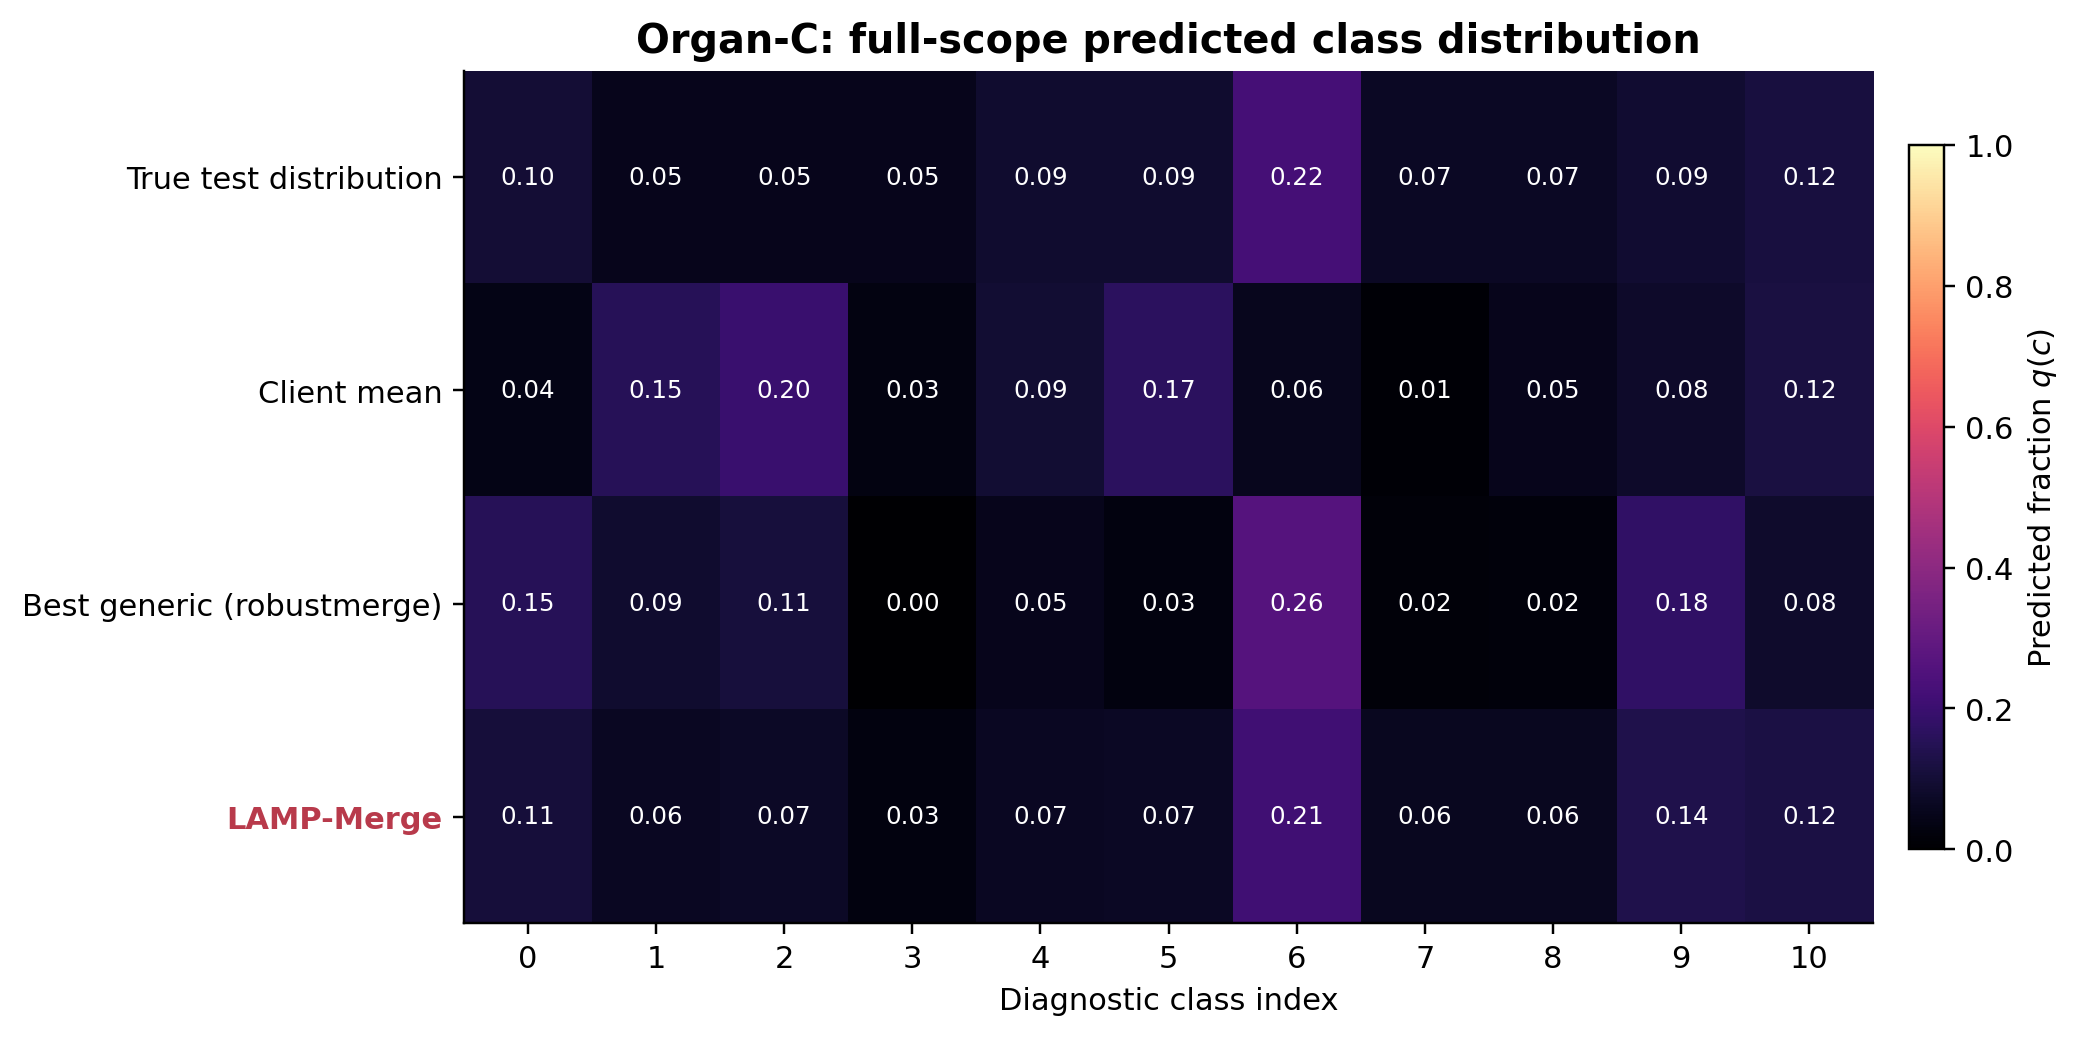
\includegraphics[width=\linewidth,keepaspectratio]{figures/image30.png}
\end{figure}

% --- DOCX block 138 ---
% Original image: image31.png
\begin{figure}[t]
\centering
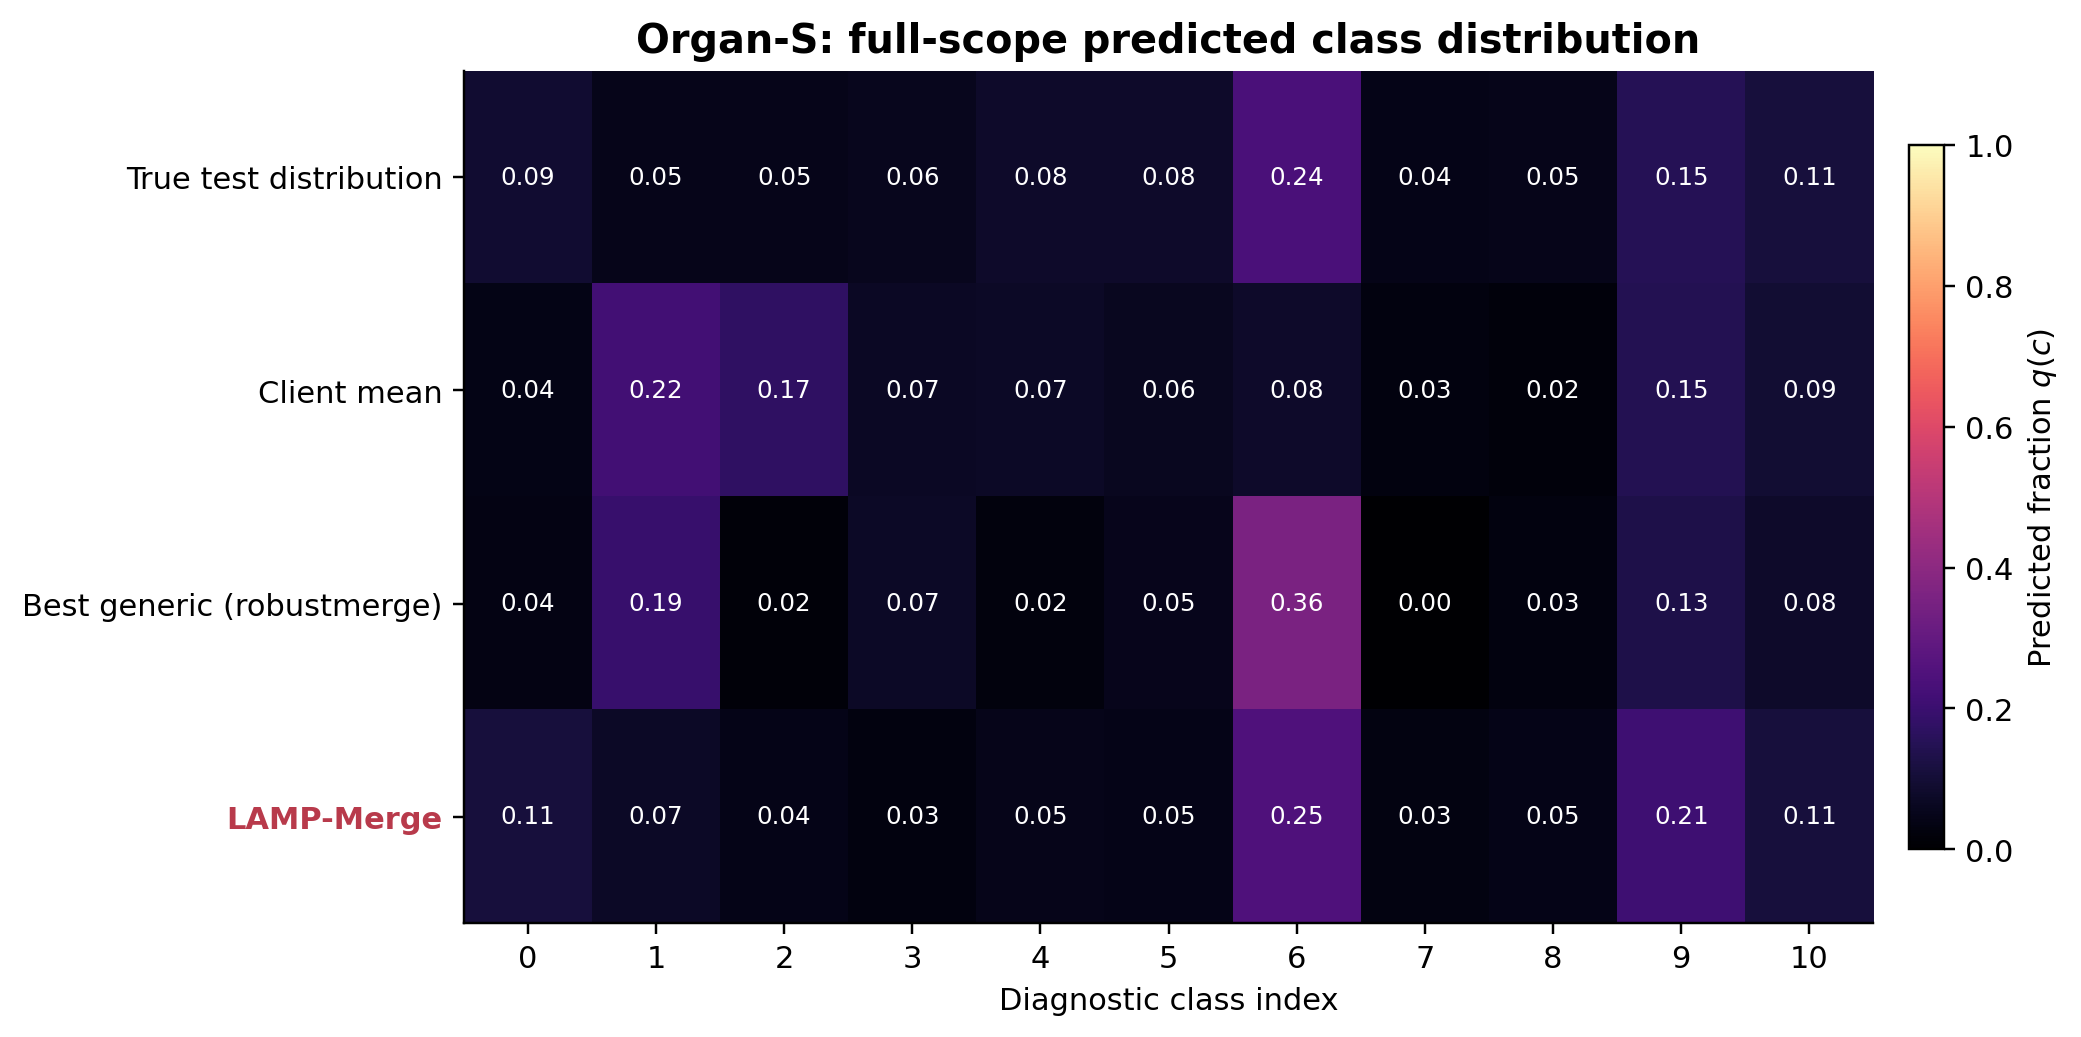
\includegraphics[width=\linewidth,keepaspectratio]{figures/image31.png}
\end{figure}

% --- DOCX block 139 ---
% Original: t-SNE
\subsection{t-SNE}

% --- DOCX block 140 ---
% Original: t-SNE 仅用于论文分析，不参与服务端融合或模型选择。对每个 (dataset, backbone)，分析将该 backbone 的测试特征与 5 个方法在全部 9 个 (K,b) 设置下的类别原型放入同一次 t-SNE 拟合；五个子图共享同一二维坐标系，因此原型位置可以跨方法比较。20 张图覆盖 5 个数据集和 4 个 backbone。
t-SNE is used only for paper analysis and does not participate in server-side merging or model selection. For each (dataset, backbone), the analysis places the test features of that backbone and the class prototypes of 5 methods under all 9 (K,b) settings into the same t-SNE fitting. The five subplots share the same two-dimensional coordinate system, so prototype positions are comparable across methods. The 20 figures cover 5 datasets and 4 backbones.


% --- DOCX block 141 ---
% Original image: image32.png
\begin{figure*}[t]
\centering
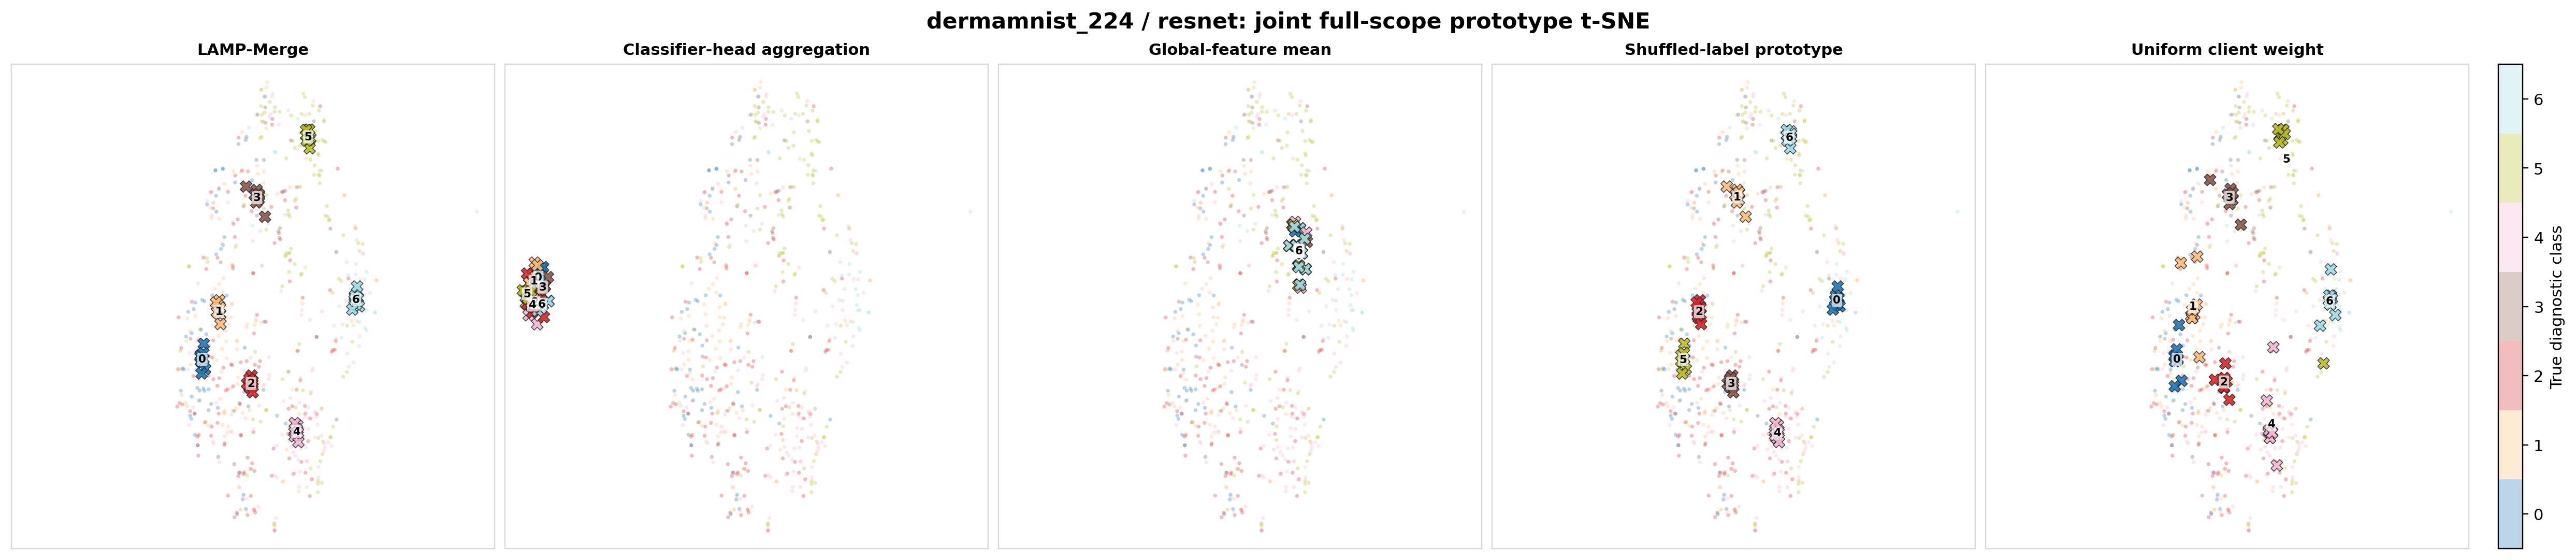
\includegraphics[width=\textwidth,keepaspectratio]{figures/image32.png}
\end{figure*}

% --- DOCX block 142 ---
% Original: 剩余的图没放进来
The remaining figures are not included.


% --- DOCX block 143 ---
% Original: 深入分析实验
\section{In-depth Analysis Experiment}

% --- DOCX block 144 ---
% Original: 该实验只利用客户端上传的类别原型、类别支持数和由这些统计量构造的全局原型。用于判断正式方法恢复多类别诊断能力，是因为原型携带了稳定的类别语义方向，还是仅仅因为增加了额外参数或统计量。
This experiment uses only the class prototypes, class support counts, and global prototypes constructed from these statistics uploaded by clients. It evaluates whether the formal method restores multi-class diagnostic ability because the prototypes carry stable class semantic directions, or merely because extra parameters or statistics are added.


% --- DOCX block 145 ---
% Original: Accuracy 消融共有 11 个设置；本节只列出 8 个会改变原型几何的设置。`No prevalence calibration`、`Uniform prevalence prior` 与 `Smoothed prevalence prior` 只改变 M2 的类别 bias $b_c$，不改变全局原型 $p_c$、客户端权重 $\alpha_{i,c}$ 或客户端类别原型 $\mu_{i,c}$，因此其几何指标与对应原型构造完全重合。将它们重复画入几何图不会提供新的几何证据。
The Accuracy ablation contains 11 settings; this section lists only the 8 settings that change prototype geometry. No prevalence calibration, Uniform prevalence prior, and Smoothed prevalence prior only change the M2 class bias $b_c$ and do not change the global prototype $p_c$, client weight $\alpha_{i,c}$, or client class prototype $\mu_{i,c}$. Therefore, their geometric metrics completely overlap with the corresponding prototype construction. Repeating them in the geometry figure would not provide new geometric evidence.


% --- DOCX block 146 ---
% Original image: image33.png
\begin{figure}[t]
\centering
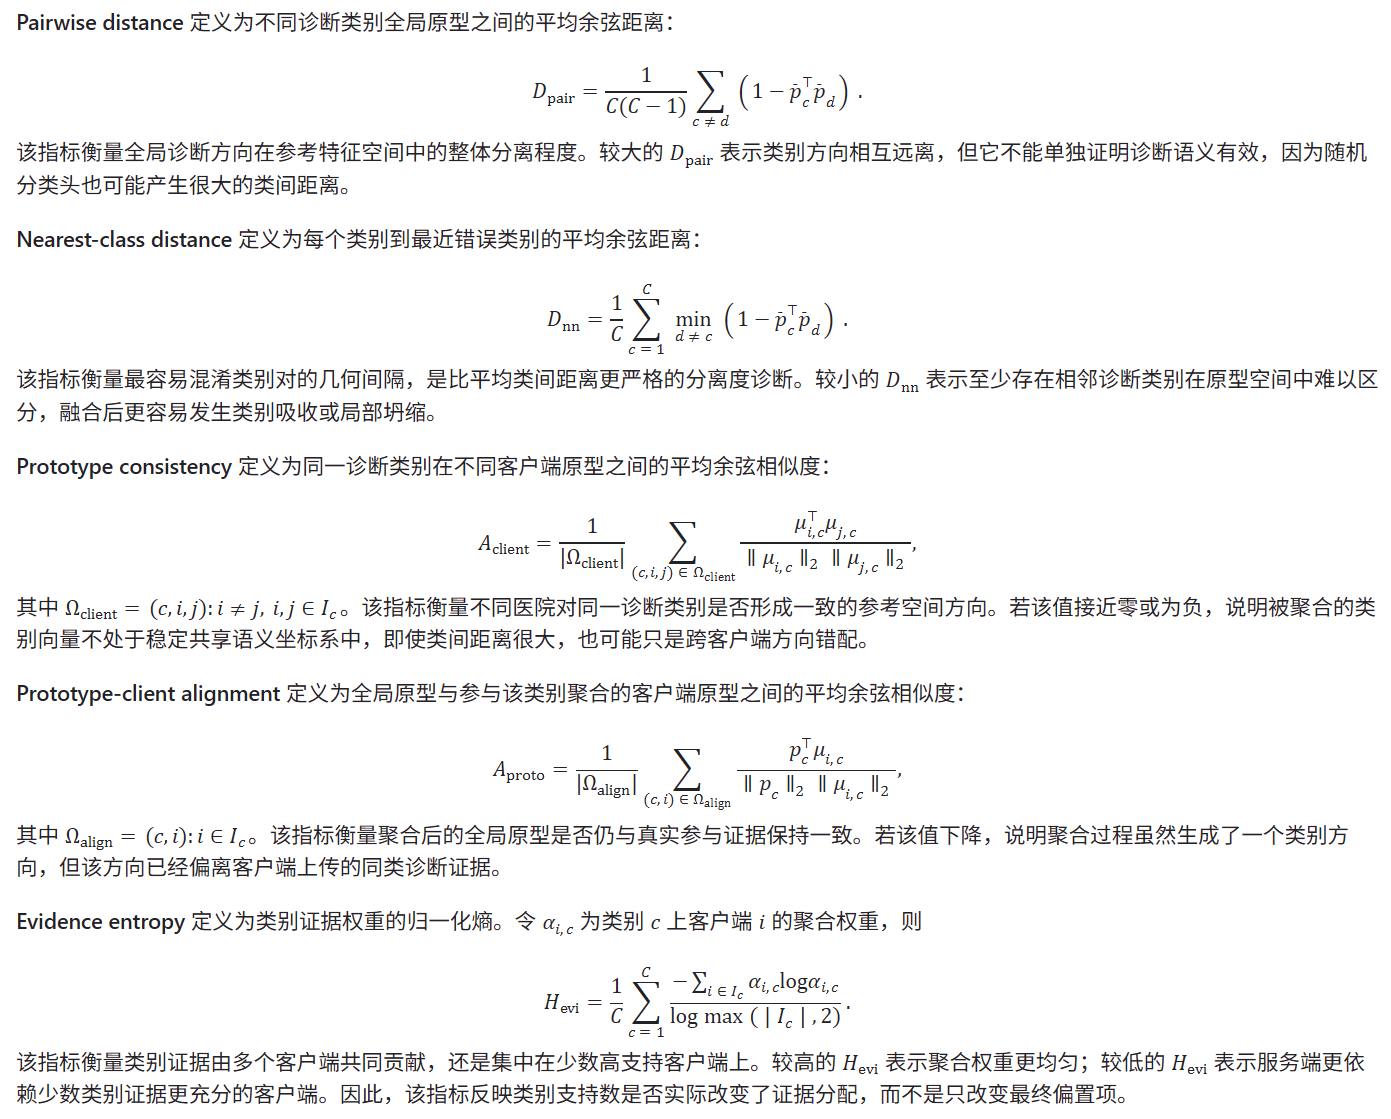
\includegraphics[width=\linewidth,keepaspectratio]{figures/image33.png}
\end{figure}

% --- DOCX block 147 ---
% Original image: image34.png
\begin{figure*}[t]
\centering
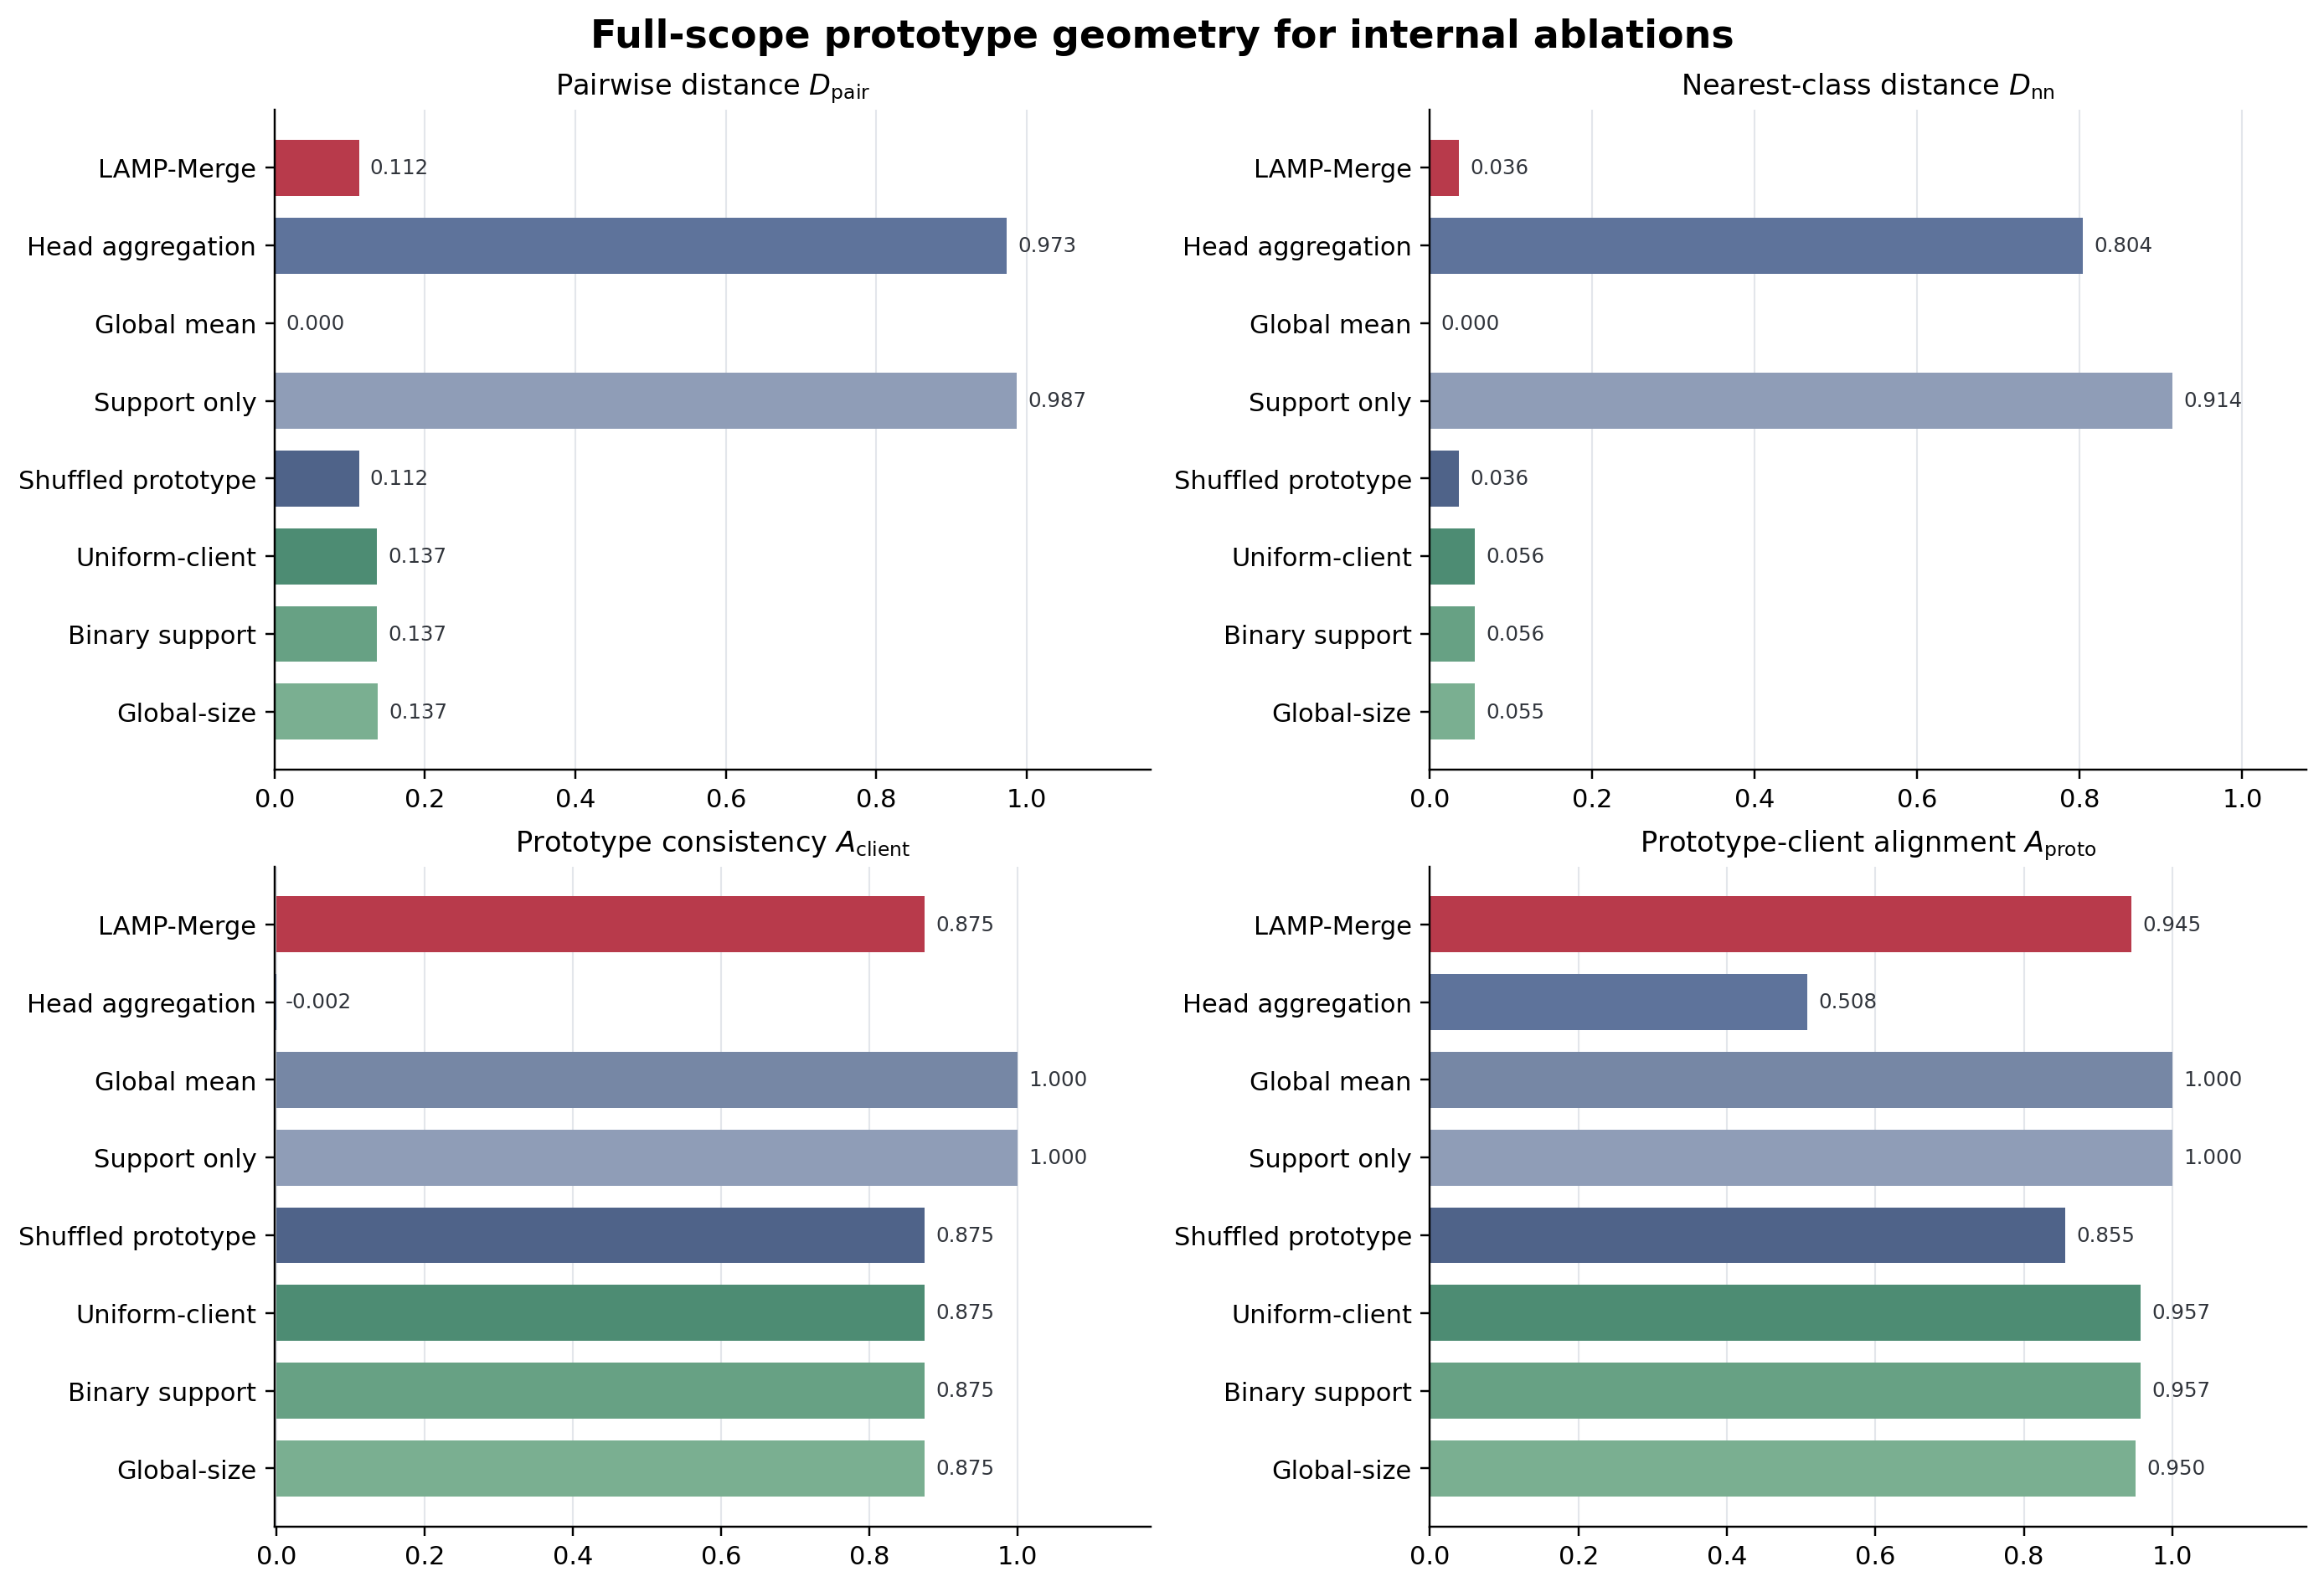
\includegraphics[width=\textwidth,keepaspectratio]{figures/image34.png}
\end{figure*}

% --- DOCX block 148 ---
% Original:     这组结果支持 LAMP-Merge 的核心机制：正式方法并不是最大化单一几何指标，而是在诊断类别可分性、跨客户端语义一致性、全局原型与客户端证据对齐、以及类别支持数驱动的证据分配之间形成稳定组合。具体而言，LAMP-Merge 在 full-grid 上保持非零的 Pairwise distance 和 Nearest-class distance，说明每个诊断类别在共享参考特征空间中具有独立判别方向；同时，Prototype consistency 达到 0.8751，Prototype-client alignment 达到 0.9446，说明这些类别方向既能在不同客户端之间保持同类语义一致，又没有在服务端聚合后偏离客户端上传的真实类别证据。Evidence entropy 为 0.2505，表明正式方法没有简单地让所有客户端等权贡献，而是根据类别支持数对更可靠的客户端证据赋予更高权重。
This group of results supports the core mechanism of LAMP-Merge: the formal method does not maximize a single geometric metric, but forms a stable combination among diagnostic class separability, cross-client semantic consistency, global-prototype alignment with client evidence, and evidence allocation driven by class support counts. Specifically, LAMP-Merge maintains nonzero Pairwise distance and Nearest-class distance on the full grid, showing that each diagnostic class has an independent discriminative direction in the shared reference feature space. Meanwhile, Prototype consistency reaches 0.8751 and Prototype-client alignment reaches 0.9446, showing that these class directions preserve same-class semantic consistency across clients and do not deviate from the real client-uploaded class evidence after server aggregation. Evidence entropy is 0.2505, indicating that the formal method does not simply assign equal contributions to all clients, but gives higher weights to more reliable client evidence according to class support counts.


% --- DOCX block 149 ---
% Original:     因此，个别消融设置在某些单项几何指标上超过 LAMP-Merge 并不构成反证。Pairwise distance 或 Nearest-class distance 过大只说明方向彼此远离，并不保证这些方向对应真实诊断语义；Prototype consistency 或 Prototype-client alignment 接近 1 也可能来自类别无关方向或构造性一致，而不代表存在有效的类别判别边界；Evidence entropy 更高则表示证据分配更均匀，但在医学长尾和客户端类别缺失场景中，均匀分配会削弱高支持客户端的可靠类别证据。换言之，这些几何量应作为联合诊断而不是独立优化目标。LAMP-Merge 的优势在于其几何结构与最终 Accuracy 消融结果一致：共享参考特征空间类别原型提供稳定的诊断语义方向，类别支持数负责可靠性加权，长尾先验只对最终分数进行有界校准。
Therefore, the fact that some ablation settings exceed LAMP-Merge on individual geometric metrics is not a counterexample. Excessively large Pairwise distance or Nearest-class distance only indicates that directions are far apart, but does not guarantee that these directions correspond to true diagnostic semantics. Prototype consistency or Prototype-client alignment close to 1 may also come from class-agnostic directions or constructive consistency, and does not imply the existence of effective class-discriminative boundaries. Higher Evidence entropy means more uniform evidence allocation, but in medical long-tail and client-class-missing scenarios, uniform allocation weakens reliable class evidence from high-support clients. In other words, these geometric quantities should be used as joint diagnostics rather than independent optimization targets. The advantage of LAMP-Merge is that its geometric structure is consistent with the final Accuracy ablation: shared reference-space class prototypes provide stable diagnostic semantic directions, class support counts perform reliability weighting, and the long-tail prior only gives bounded calibration to the final scores.


% --- DOCX block 150 ---
% Original: 理论分析补充
\section{Additional Theoretical Analysis}

% --- DOCX block 151 ---
% Original image: image35.png
\begin{figure}[t]
\centering
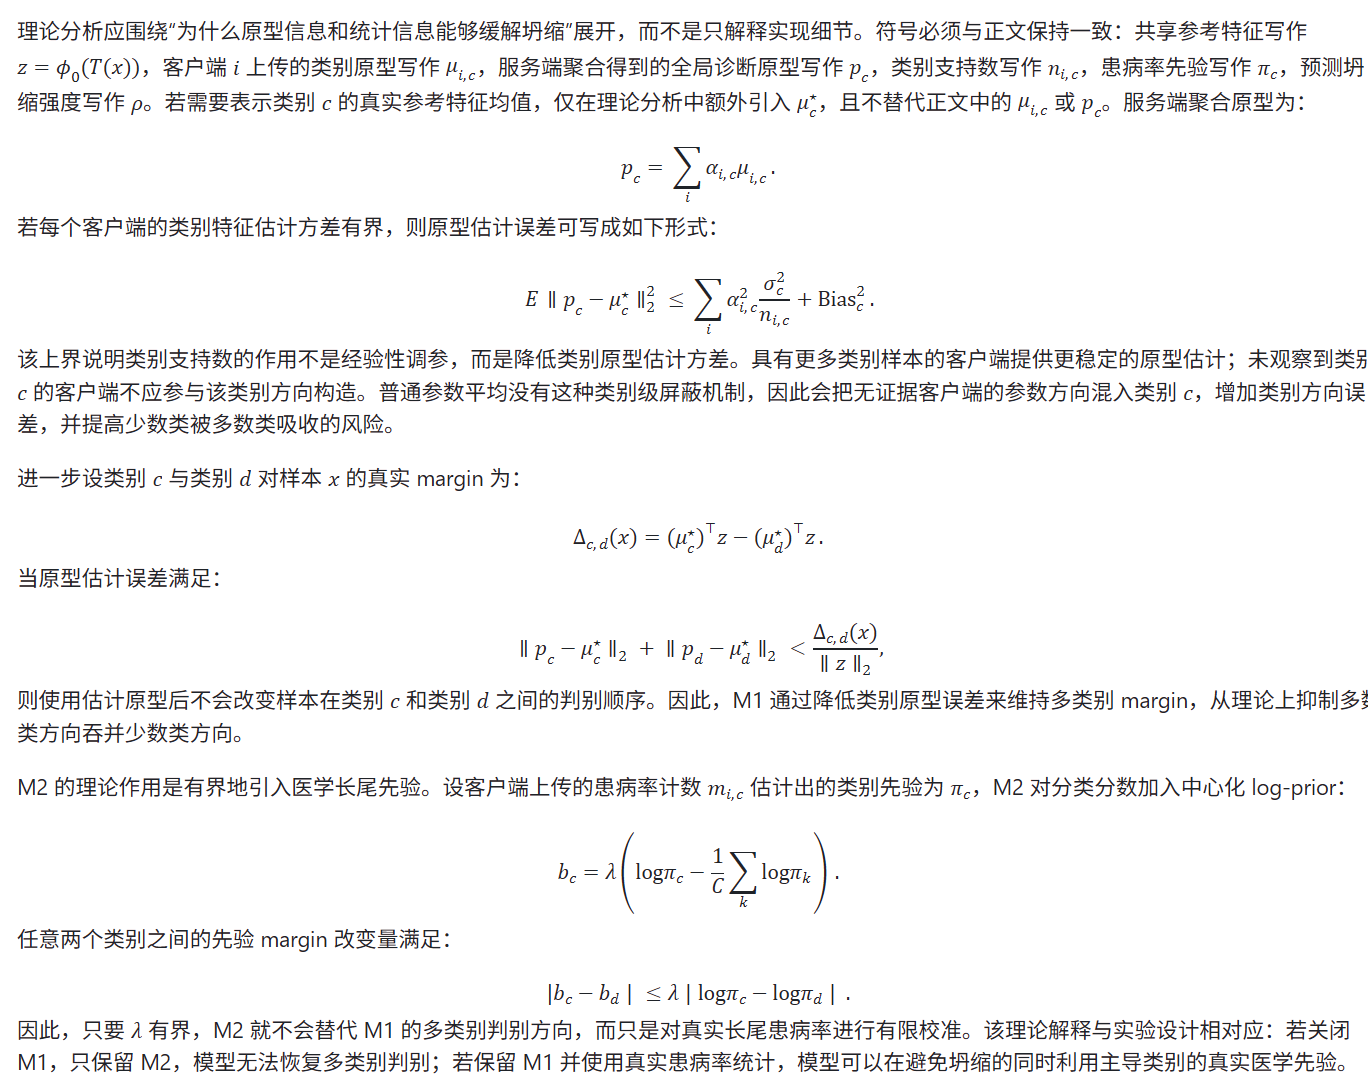
\includegraphics[width=\linewidth,keepaspectratio]{figures/image35.png}
\end{figure}

\end{document}
